\chapter{Estabilidad del sistema de Lotka-Volterra generalizado}

\setlength{\parindent}{0cm} El capítulo anterior motiva al actual para presentar los resultados de la dinámica que produce el sistema de Lotka-Volterra generalizado (\ref{eqn:LK}) bajo los coeficientes de interacción de la matriz de incidencias (\ref{eqn:MatrizIncidencias}) para posteriormente linearizarlo mediante la Matriz Jacobiana del sistema (\ref{eqn:MartizJacobiana}). En este capítulo se presentarán los resultados que produce cada etapa del proceso, así como sus características. El objetivo será dar respuesta a cada una de las hipótesis del planteamiento del problema, sobre todo indagar las condiciones de estabilidad del sistema en términos de $\Lambda$ y reforzar la idea consecuente de la proposición \ref{prop:paramMay} en la que se detallaba que el parámetro de May (\ref{eqn:radioMayGirko}) no necesariamente se ajusta a la estabilidad del sistema de Lotka-Volterra.\\
\\
Se consideraron 3 conjuntos diferentes de simulaciones: sistemas para 25, 50 y 100 especies. Para explorar los resultados se dejaron fijos la mayor cantidad de parámetros que hay en (\ref{eqn:LK}) con el fin de observar cambios significativos con la menor cantidad de fluctuaciones posibles; únicamente se han variado las matrices de incidencias $\Lambda$ que dependen de $p$ y $\sigma$, y al igual que en las transiciones de May se varió una de estas cantidades mientras que la otra permaneció fija. En todas las simulaciones la tasa de crecimiento se dejó fija en $r=2$ y la capacidad de carga en $K=5$ para toda especie del sistema. Al integrar numéricamente las ecuaciones con RK4 se escogió un intervalo de tiempo entre 0 y 50 con un paso de integración de $h=0.01$.\\
\\
Además de estos parámetros, siempre se inicializó cada simulación con la condición inicial $\vec{x}_0=\vec{1}$ (según el tamaño del sistema) y se consideraron dos escenarios\footnote{solo aplicca para $N=100$, el resto de casos se consideraron $\Lambda$ estructuralmente simétricas.}: Matrices de incidencias estructuralmente simétricas y puramente aleatorias, tal y como se visualizó al final del capítulo anterior. En el apéndice (\ref{ch:Ap}), el lector puede darse una idea de como se realizó el proceso de las simulaciones. En cada escenario se presentó cierta cantidad de ruido en las gráficas de estabilidad, por lo que el número de simulaciones fue establecido en función de la disminución de dicho ruido (haciendo uso de la ley de los grandes números).

\section{Series de tiempo}

Anteriormente se ha comentado que las interacciones de la matriz de incidencias $\Lambda$ están volteadas con respecto de la matriz de Jacobiana del sistema $\mathcal{J}$; por ejemplo, la cooperación en $\mathcal{J}$ se da para las interacciones (++) mientras que para $\Lambda$ es $(--)$. La propia definición de la Jacobiana garantiza este hecho. Si se tuviera un sistema puramente de competencia, es decir para toda $\alpha_{ij}\in\Lambda$ mayor o igual que cero, entonces no hay forma de que ninguna de las poblaciones participantes sobrepasen la capacidad de carga establecida, tal y como se indica en la ecuación (\ref{eqn:LKextendida}) y en el Ejemplo \ref{eg:2x2}. Por lo tanto obtendríamos series de tiempo caóticas para cada una de las especies por debajo de $K=5$.
\begin{figure}[h!]
	\centering
	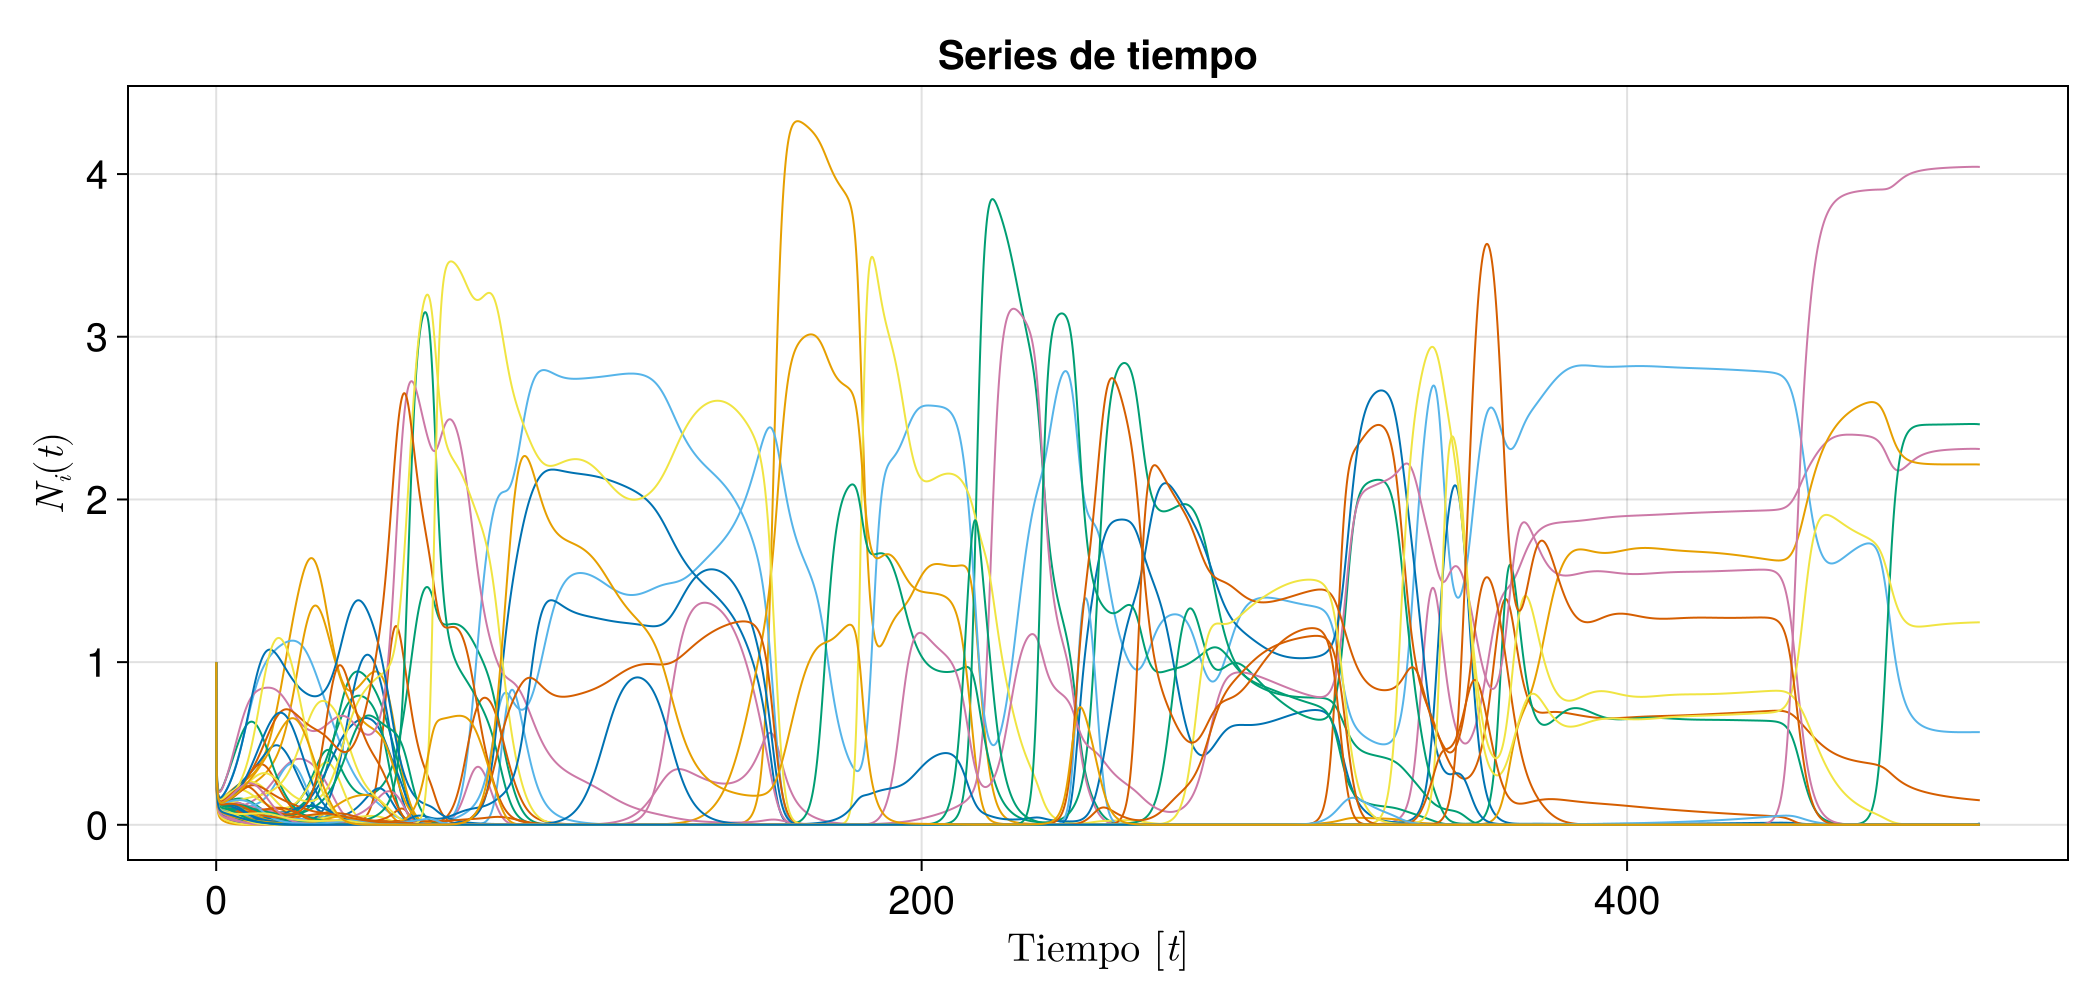
\includegraphics[scale=0.23]{../Imagenes/Seriesdetiempopositiva}
	\caption{Series de tiempo para el sistema de competencia de especies. Se emplea una matriz de incidencias para $N=100$ cuyas entradas vienen de una distribución uniforme del intervalo $[0,1]$. Se considera a la red completa con $p=1.0$, es decir, con el número máximo de enlaces posibles. En este caso la dinámica no sobrepasa la capacidad de carga puesto que las 100 especies se encuentran compitiendo y obedeciendo el comportamiento logístico que se muestra en (\ref{eqn:LKextendida}).}
	\label{fig:Seriesdetiempopostiva}
\end{figure}

Una de las características que se encontró en esta clase de sistema en particular es que el tiempo en que tarda en estabilizarse es considerablemente mayor que en los sistemas donde se considerarán todas las interacciones antes mencionadas. Las poblaciones al estar confinadas por la capacidad de carga, tienen más oportunidad de interactuar entre sí, generando constantes fluctuaciones que prolongan el tiempo de estabilización.\\
\\
Por el contrario, el sistema generalizado sí excede la capacidad de carga lo que se traduce en una disminución de la cantidad de fluctuaciones debido a las especies dominantes que regulan el sistema y hace que lleguen al atractor en un tiempo menor. Otro aspecto que se encontró en la red de competencias es que cuando es más conectada tarda más tiempo en estabilizarse. Si se generara una red de competencias con pocas conexiones ($p\leq 0.5$) el número de especies que compiten es considerablemente menor, lo que implica que exista menor cantidad de fluctuaciones y por ende mayor facilidad para llegar a la estabilidad.\\
\\
En el Ejemplo \ref{eg:2x2CoopyDemás} del capítulo anterior, se observaba como las interacciones de cooperación $(--)$ en la matriz de incidencias $\Lambda$ genera la aparición de un atractor para ambas especies que se posiciona por arriba de la capacidad de carga (Figura (\ref{fig:CooperacionEspecies})). En el caso extendido a $N\gg 1$ especies ocurrirá algo semejante considerando un atractor $N$-dimensional. En este caso pueden haber especies que sobrepasen por mucho o poco la capacidad de carga, pero también cabe la posibilidad de que algunas no logren sobrepasarla y otras que lleguen a extinguirse. A continuación se muestran dos ejemplos diferentes
\begin{figure}[h!]
	\centering
	\includegraphics[scale=0.23]{../Imagenes/Series de Tiempo LK100}
	\caption{(\textbf{A}) Series de tiempo del sistema de Lotka-Volterra generalizado asociada a una matriz de incidencias de $N=100$, con $\sigma=0.2$ y $p=0.35$. (\textbf{B}) Series de tiempo para el sistema de Lotka-Volterra generalizado asociada a una matriz de incidencias de $N=100$ nodos con $\sigma=0.2$ y $p=0.5$}
	\label{fig:SeriesdeTiempoLK100}
\end{figure}

La diferencia evidente entre estas gráficas es debido la matriz de incidencias, sus parámetros son $\sigma=0.2$ con $p=0.35$ y $p=0.5$ respectivamente. El segundo caso corresponde con una red más conectada que el primero y eso se traduce en la oportunidad de tener más interacciones con signo negativo que propicien un mayor crecimiento. El tiempo en que llegaron a estabilizarse fue menor a $t=50$, y a su vez considerablemente menor que el sistema de competencia de especies de la Figura (\ref{fig:Seriesdetiempopostiva}). 
\\
\\
En un principio, los resultados de la Figura (\ref{fig:SeriesdeTiempoLK100}) se generaron sin tener un mapa de estabilidad únicamente teniendo como referencia el parámetro de May (\ref{eqn:radioMayGirko}). Además de construir los mapas de estabildiad (que es lo que se hará más adelante), es de interés buscar un parámetro crítico de transición como el de May. Para ello será crucial conocer más sobre $\Lambda$, pues es quien realmente determina la estabilidad de los sistemas.

\subsection{Puntos fijos}\label{subsec:PuntosFijos}

Como bien ya se sabe, los puntos fijos son aquellos en los que se refleja la estabilidad del sistema además de que son vitales para determinar la matriz Jacobiana del sistema de Lotka-Volterra generalizado. Sin embargo, serán los propios coeficientes de la matriz de incidencias los que definan si el sistema es estable o no. Esta conjetura podrá no ser trivial de abordar pero si es posible realizar un análisis exploratorio. Los puntos fijos del sistema se determinan de igualar a cero y resolver las ecuaciones (\ref{eqn:LK}) lo que sería equivalente tener el siguiente sistema
\begin{equation}\label{eqn:PuntoFijo}
	x_i=K_i-\sum_{j\neq i}\alpha_{ij}x_j,\qquad\alpha_{ij}\in\Lambda
\end{equation}
considerando que $\alpha_{ii}=1$. Las soluciones que puede tener este sistema son múltiples, se pueden generar combinaciones de casos para poder resolverlo: por ejemplo igualar a cero un subconjunto de ecuaciones de este sistema ($x_{k}=0$) y resolver para dicha/s condición/es. Las soluciones favorables son para cuando todo elemento $x_i\in X$ del punto fijo es mayor o igual que cero; el sistema no restringe soluciones $x_k\in X$ negativas, pero no serán de interés puesto que no hay sentido físico en interpretar poblaciones negativas\footnote{Además de que los experimentos han arrojado sistemas inestables cuando el punto fijo $X$ tiene entradas negativas.}. Por último, de las soluciones favorables es de interés saber que condiciones en $\Lambda$ hace que el punto fijo sea estable o inestable.\\
\\
Para un primer análisis exploratorio, se utilizará aproximación de campo medio para realizar una estimación general de las soluciones del sistema. Para ello se considerará que toda $x_i\in\Lambda$ cumple $x_i\approx\langle x\rangle$, asumiendo esta hipótesis y aplicándola en (\ref{eqn:PuntoFijo}) se tiene
\begin{equation}
	\begin{split}
		&\langle x\rangle+\sum_{j\neq i}\alpha_{ij}\langle x\rangle=K_i\\
		&\langle x\rangle=\frac{K_i}{1+pN\sigma^2},\qquad 
	\end{split}
\end{equation}
considerando que $\sum_{j\neq i}\Var(\alpha_{ij})\approx pN\sigma^2$. Este resultado indicaría como son las soluciones del punto fijo en gran o en menor medida, de aquí en adelante se tendría el camino directo para poder estimar el parámetro de transición que tanto se espera sino fuera por algunos aspectos a considerar: La suposición de campo medio excluye soluciones negativas, lo cual se sabe que existen pero para ningún valor de $p$, $N$ y $\sigma$ se generan tales escenarios; el segundo aspecto a considerar es que de acuerdo a los ejemplos de la Figura (\ref{fig:SeriesdeTiempoLK100}), el punto fijo no sigue una distribución de campo medio, sino más bien una tendencia de distribución de cola pesada con sesgo positivo. \\
\\
El lector podrá comprobarlo una vez que haya seguido todos los pasos del apéndice para integrar el sistema. Además podrá comprobar que dicha distribución irá variando en función de los parámetros de $\Lambda$ lo cual también se deja ver un poco en las series de tiempo mencionadas. Una alternativa para poder estimar una solución tal y como se hacía considerando aproximación de campo medio sería adecuar este proceso para la distribución de cola pesada. Suponer campo medio es considerar que las entradas del punto fijo siguen una distribución normal, la idea en este caso sería caracterizar estas distribuciones de cola pesada con alguna ya conocida y aplicar campo medio bajo la hipótesis de esta nueva distribución.\\
\\
Teniendo contexto de la distribución de las entradas del punto fijo (mediante las series de tiempo generadas) y de los coeficientes de $\Lambda$ que inducen a dicha distribución, se podrá acceder a la información necesaria para determinar que condiciones generan sistemas de Lotka-Votlerra generalizados estables. Pero por el momento el análisis quedará hasta aquí esperando que las ideas se retomen más adelante.

\section{Matriz Jacobiana}

Anteriormente se ha definido la matriz Jacobiana del sistema de Lotka-Volterra generalizado (\ref{eqn:MartizJacobiana}), para que surta efecto es necesario conocer el punto fijo de interés y se hará por medio de la serie de tiempo tal y como aparece en la Figura (\ref{fig:SeriesdeTiempoLK100}). Se recolecta la última entrada de la serie, asumiendo que es un punto fijo estable, y se guarda como vector $N$-dimensional para poderse evaluar en la matriz Jacobiana. Para validar el resultado solamente resta calcular sus valores propios y confirmar la estabilidad por medio de la parte real de los mismos. Por otro lado, si la serie de tiempo diverge entonces se asume que el sistema es inestable.
\\
\\
Un elemento importante de este proceso es que no es trivial determinar cuando se estabilizará el sistema por medio de la serie de tiempo, en general se ha observado que gran porcentaje de los sistemas se estabilizan en un tiempo menor o igual a $t=50$, sin embargo, existen sistemas que se estabilizan en un tiempo superior a este lo que ha generado algunos detalles en los resultados obtenidos. En este sentido, se han observado casos en los que se extrae el punto fijo que aparenta ser estable pero al determinar la estabilidad por medio de los valores propios de la matriz Jacobiana se encuentra que  algunos de ellos tienen parte real positiva lo que induce a sistemas inestables. Para evitar que esto ocurra es importante incluir una restricción sobre el tiempo de integración, recolectar sistemas que se estabilicen en un tiempo menor o igual a $t=50$.
\\
\\
Comenzando con el análisis de los resultados obtenidos, se han generado cuatro ejemplos arbitrarios para ir observando las características de las matrices Jacobianas de los sistemas (\ref{eqn:LK}) que resultaron estables. En este \href{https://github.com/rogve98/Tesis/tree/master/Notebooks/Datos/Ejemplo\%20Jacobianos}{enlace}\footnote{Consultar: \url{https://github.com/rogve98/Tesis/tree/master/Notebooks/Datos/Ejemplo\%20Jacobianos}} el lector tendrá acceso a 4 de estas matrices para los parámetros $N=100$, $\sigma=0.2$ y $p=\{0.3,0.4,0.5,0.6\}$. A continuación se presenta el código en \julia para validar si las diagonales de cada matriz Jacobiana son negativas siguiendo la Poposición \ref{prop:DiagonalI}
\begin{tcolorbox}[colback=green!10!white, colframe=black, title=Entrada]
	\begin{minted}{julia}
		using CSV, DataFrames
		jacobianos = []
		for i in 0.3:0.1:0.6
		ruta = "Datos/Ejemplo Jacobianos/Jacobiano100_p$i.s0.2.csv"
		df = CSV.read(ruta,DataFrame,header=false)
		push!(jacobianos,df)
		end
		jacobianos
	\end{minted}
\end{tcolorbox}

\begin{tcolorbox}[colback=red!10!white, colframe=black, title=Salida]
4-element Vector{Any}:\\
100×100 DataFrame
\end{tcolorbox}

Validando las diagonales de cada uno de las matrices consideradas se tiene

\begin{tcolorbox}[colback=green!10!white, colframe=black, title=Entrada]
	\begin{minted}{julia}
using LinearAlgebra
print(all(x -> x<0,diag(Matrix(jacobianos[1]))),", ")
print(all(x -> x<0,diag(Matrix(jacobianos[2]))),", ")
print(all(x -> x<0,diag(Matrix(jacobianos[3]))),", ")
print(all(x -> x<0,diag(Matrix(jacobianos[4]))))
	\end{minted}
\end{tcolorbox}

\begin{tcolorbox}[colback=red!10!white, colframe=black, title=Salida]
true, true, true, true
\end{tcolorbox}
\newpage
El siguiente detalle a analizar siguiendo la definición de la matriz Jacobiana (\ref{eqn:MartizJacobiana}) es que sus diagonales en efecto no son homogéneas como en las matrices de May. Determinando un histograma de cada una de las diagonales de las matrices antes consideradas se puede saber como es su distribución y si cambia con respecto de la $p$ elegida
\begin{figure}[h!]
	\centering
	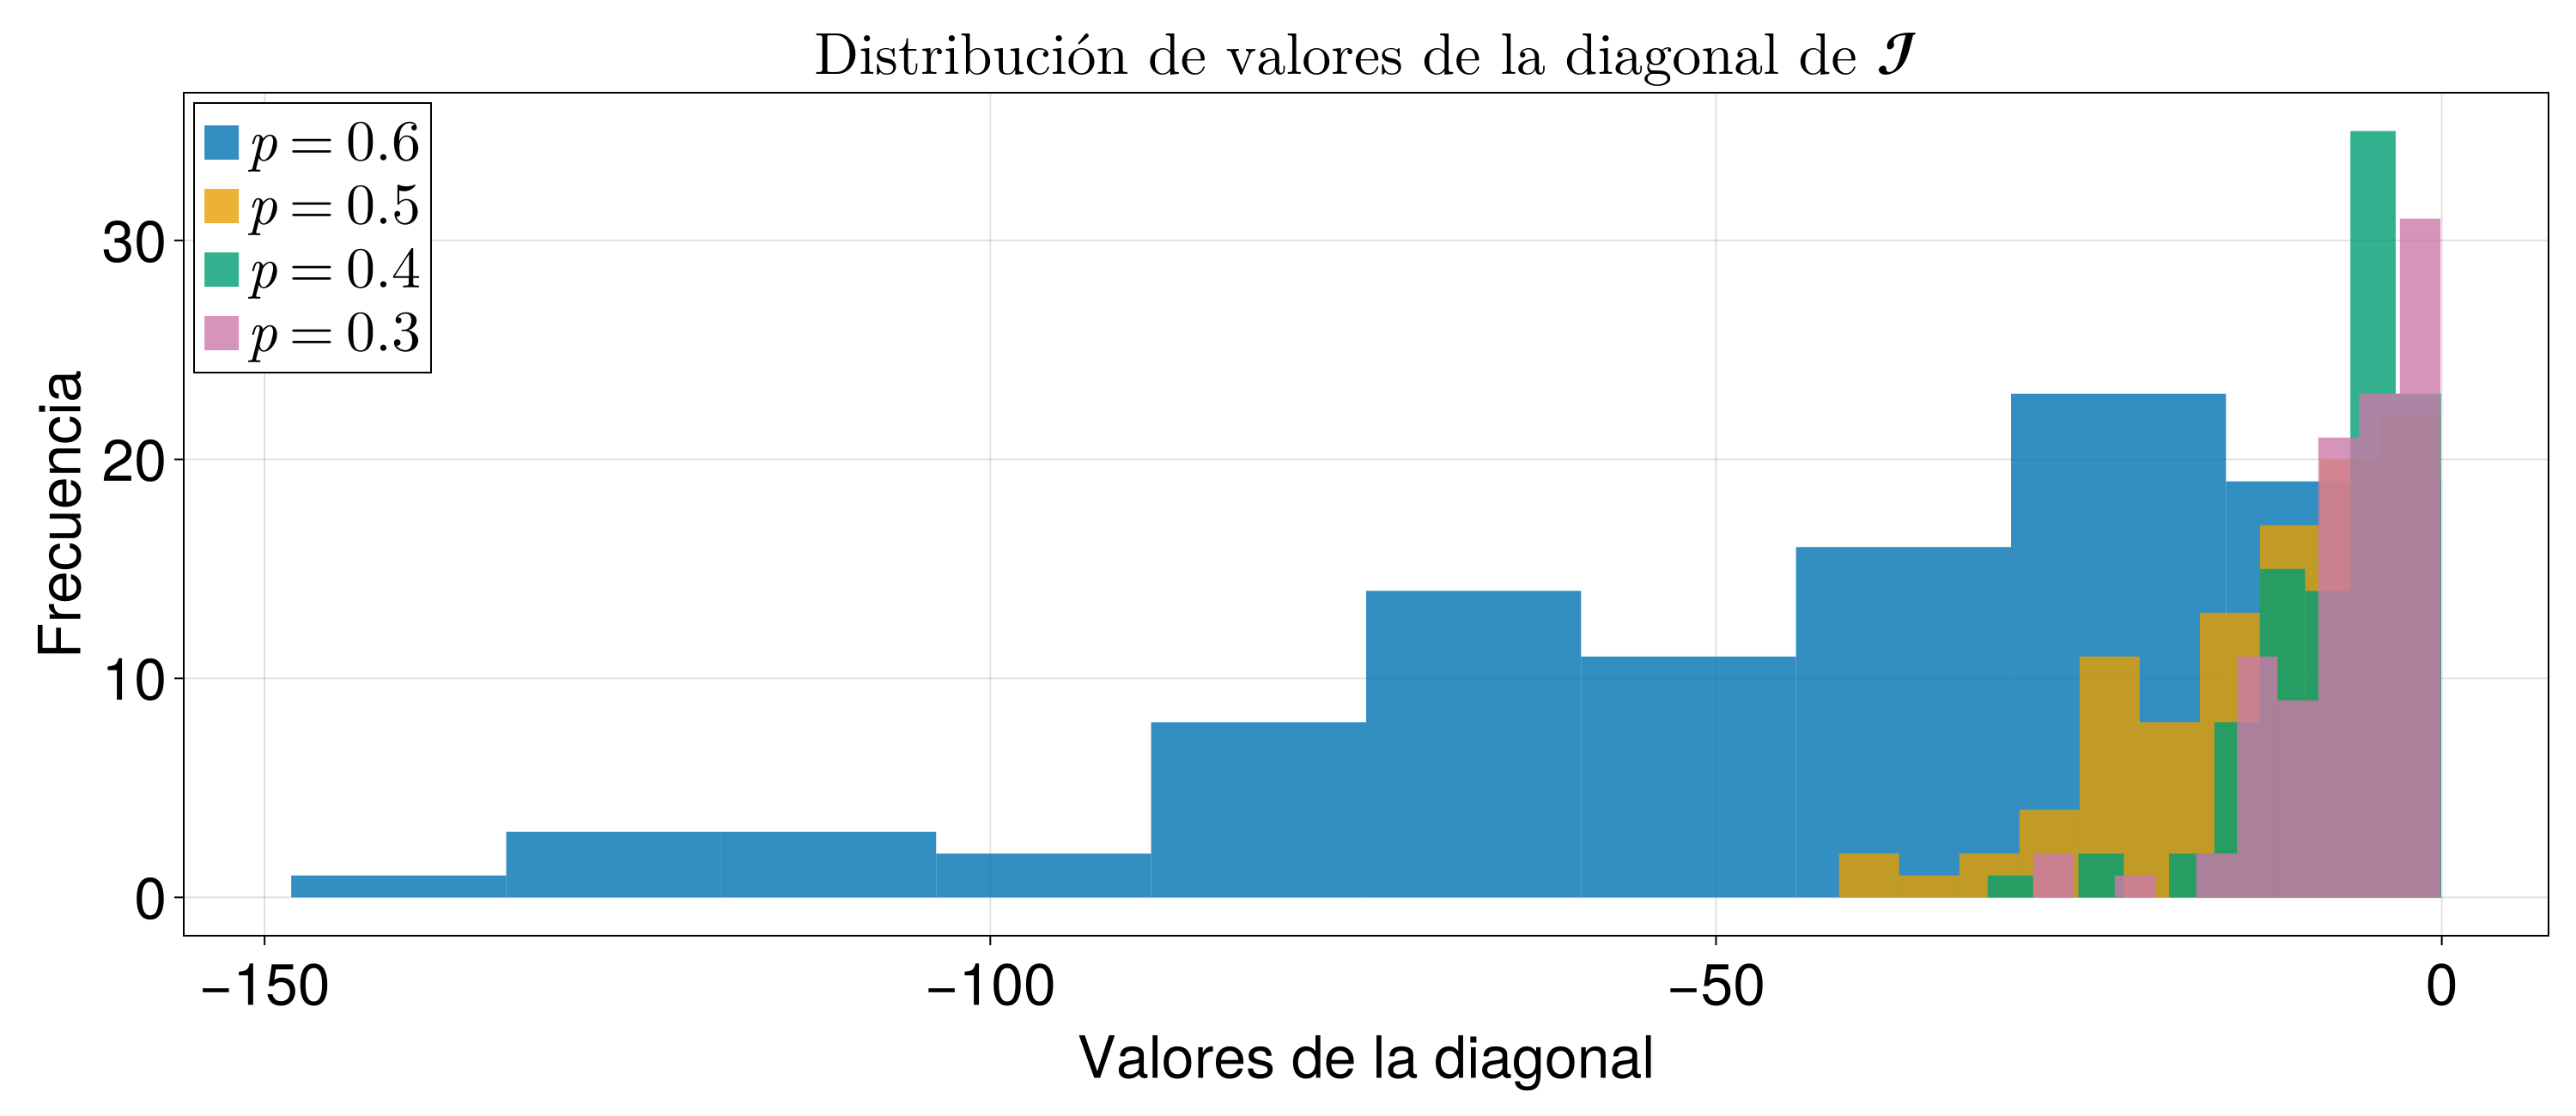
\includegraphics[scale=0.16]{../Imagenes/DistDiagonal}
	\caption{Distribuciones de diagonales de cada matriz Jacobiana antes considerada considerando para $N=100$, $\sigma=0.2$ y $p\in\{0.3,0.4,0.5,0.6\}$.}
	\label{fig:DistDiagonal}
\end{figure}

No solo no es homogénea sino que cuanto la probabilidad es mayor, la distribución es más dispersa hacia los valores negativos haciéndola de cola pesada tal como se observa el contraste entre el caso $p=0.6$ y $p=0.3$. Este comportamiento es natural considerando los coeficientes de $\Lambda$ y las entradas del punto fijo que también vienen de una distribución de cola pesada. Más adelante se discutirá acerca de esta cualidad de las distribuciones resultantes.
\\
\\
En el capítulo pasado se vio que la importancia de la diagonal en las matrices de May radica en la forma de la distribución de los valores propios del sistema en el plano complejo, englobado bajo la Ley Circular. En la Proposición \ref{prop:paramMay} se demostró que existen varios discos de Gershgorin centrados en este valor $-d$ de la diagonal, que encierran a los valores propios del sistema en el semiplano negativo de $\mathbb{C}$ y que el parámetro de May (\ref{eqn:radioMayGirko}) determina el límite entre estabilidad e inestabilidad. En el caso de las matrices Jacobianas de los sistemas de Lotka-Volterra generalizado, al no tener un radio/centro definido debido a forma heterogénea de las diagonales ¿qué se puede esperar de la distribución de valores propios de $\mathcal{J}$?
\newpage

\section{Leyes Circulares}

Sabiendo que la distribución de la diagonal de las Jacobianas de los sistemas generalizados no es homogénea y que sigue una distribución de cola pesada con sesgo negativo, se debe analizar como es su distribución de valores propios en el plano complejo y si tiene alguna relación con la distribución de la diagonal. Para ello se comenzará por revisar la distribución de los valores propios de las matrices Jacobianas que se invocaron en la sección anterior
\begin{figure}[h!]
	\centering
	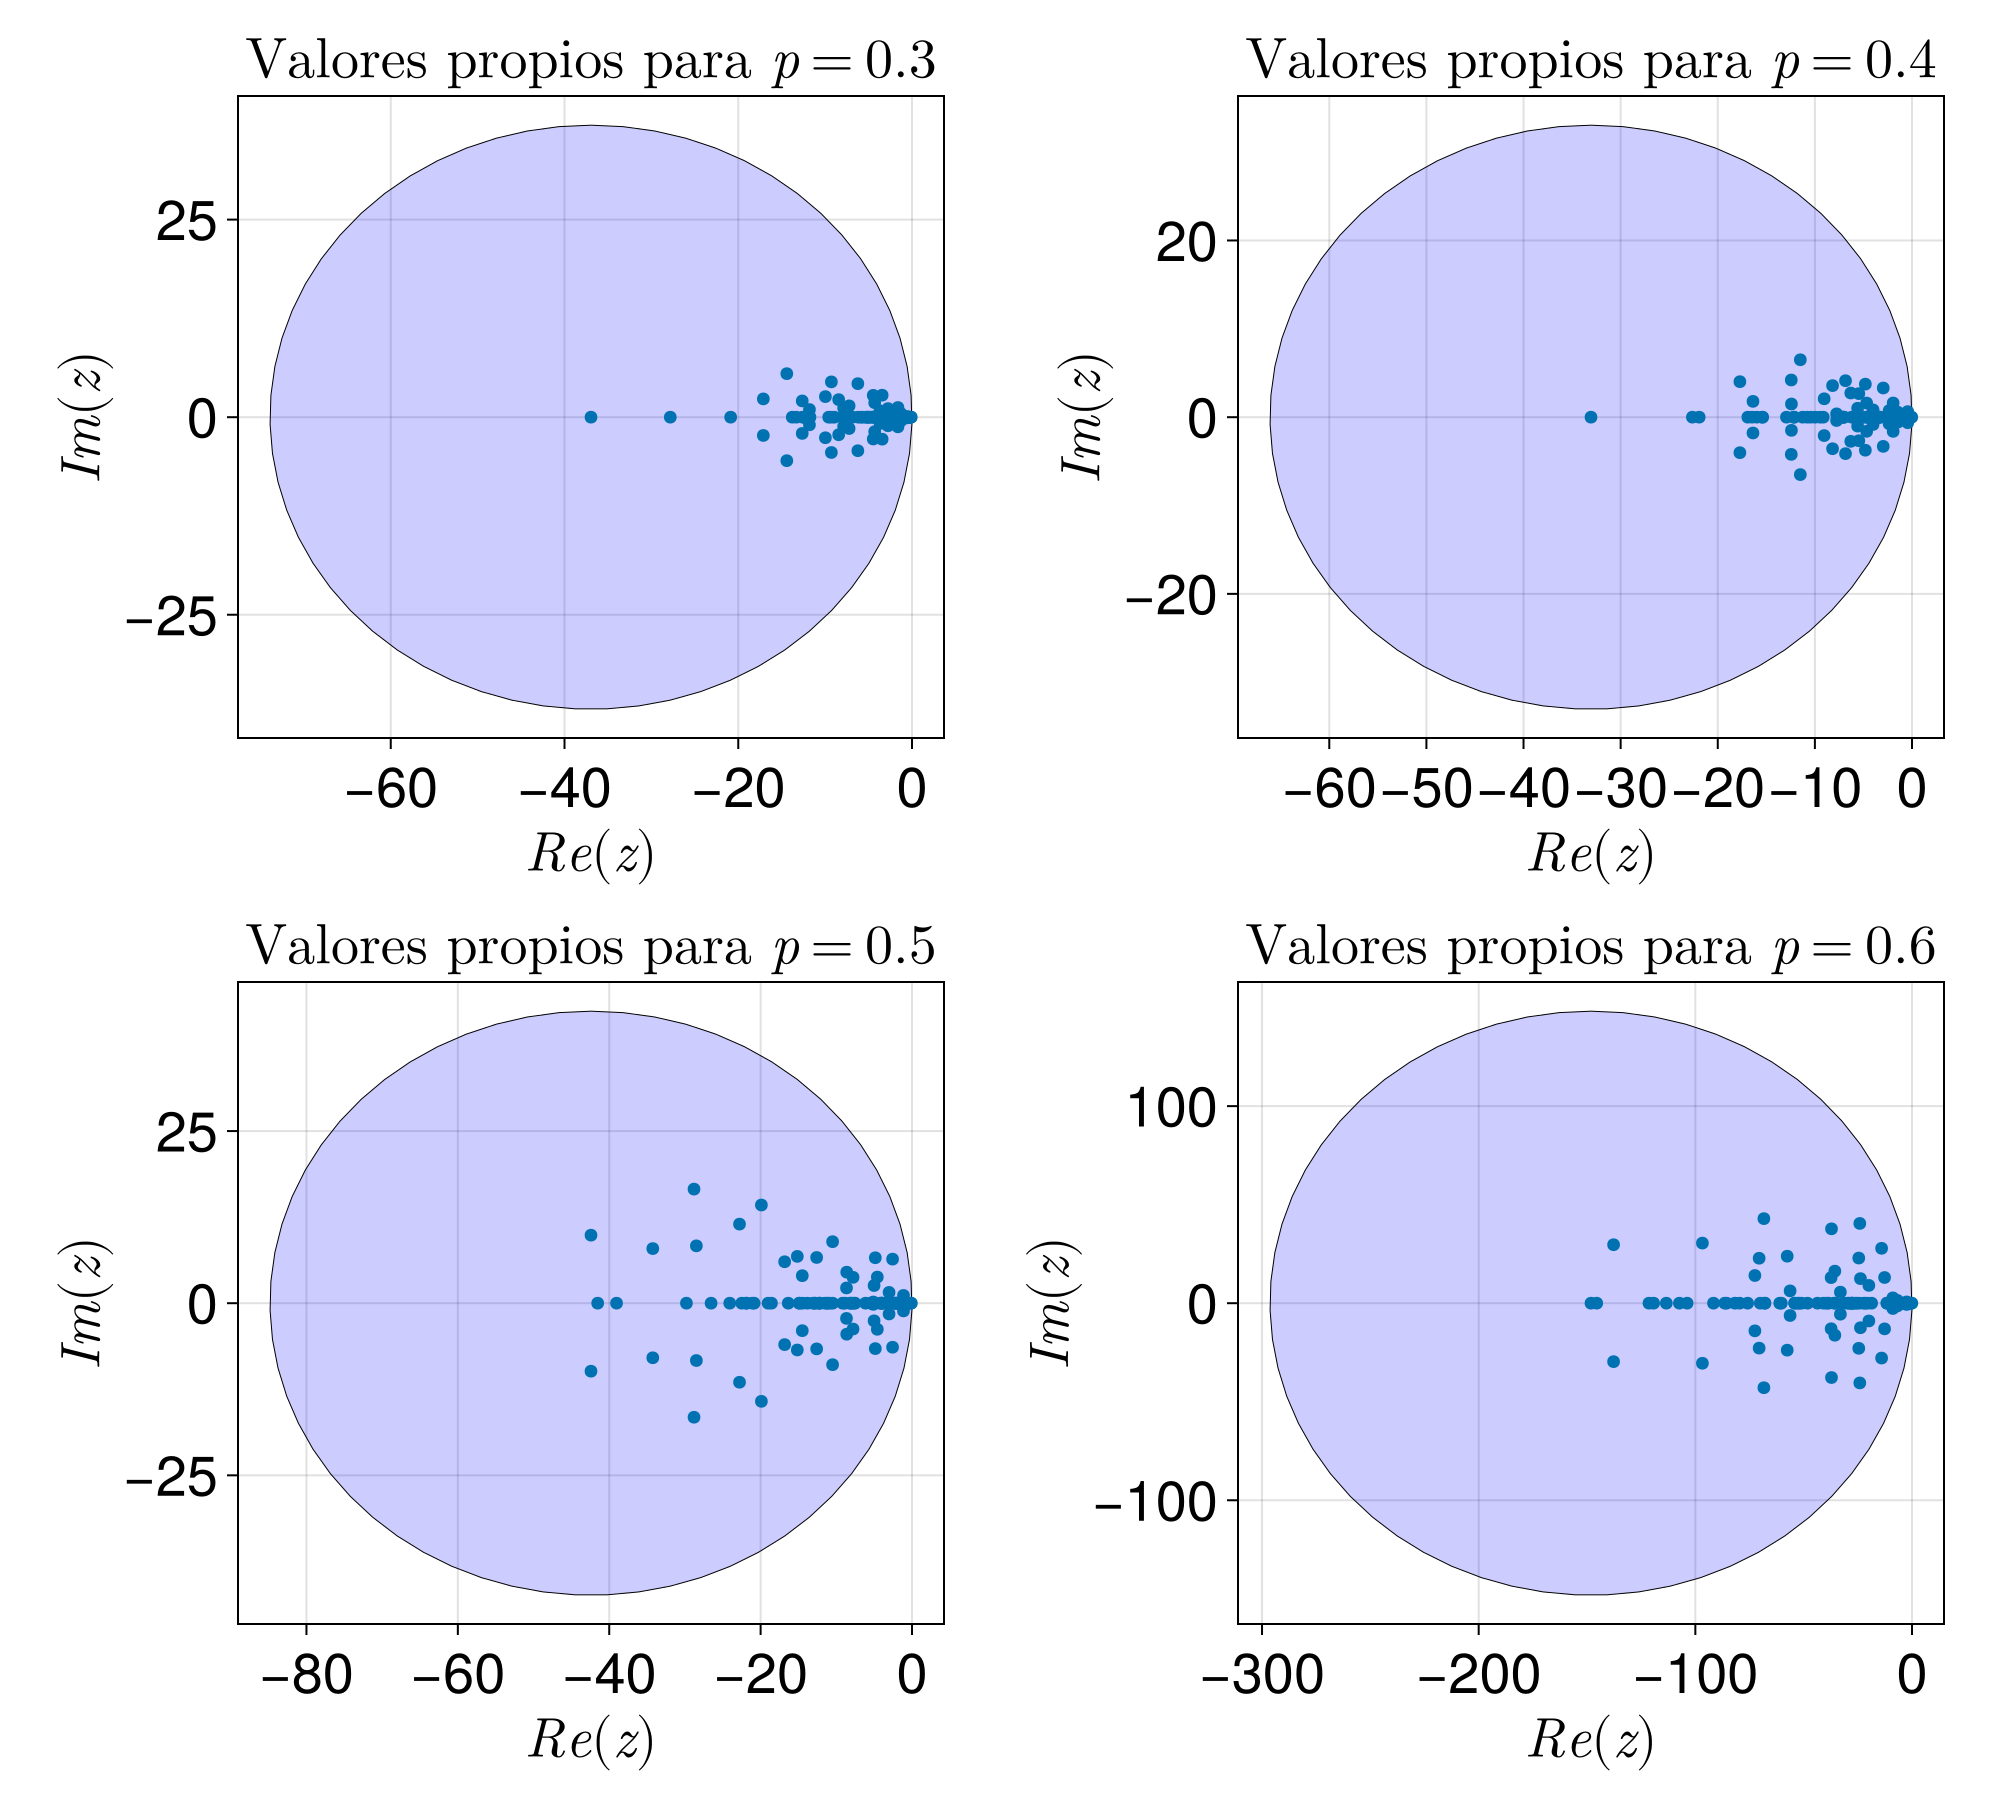
\includegraphics[scale=0.24]{../Imagenes/DistEigenvalores}
	\caption{Distribución de valores propios para el conjunto de Jacobianas antes consideradas con los parámetros $N=100$, $\sigma=0.2$ y $p\in\{0.3,0.4,0.5,0.6\}$.}
	\label{fig:DistEigenvalores}
\end{figure}

Para comenzar se han propuesto como centro y radio la parte real más negativa del conjunto de valores propios de cada ejemplo\footnote{En consecuencia se genera el Círculo con el radio más grande posible de cada sistema.}, y en primera instancia se puede observar que dichos círculos si encierran a cada una de las distribuciones pero no se ajustan al círculo en concreto. Además de que cada distribución se encuentra en el semiplano negativo de $\mathbb{C}$, se puede apreciar de cada distribución que cuando la probabilidad de conexión es mayor entonces  la distribución se ensancha desde el eje real de forma similar a como se observa en la Figura (\ref{fig:DistDiagonal}), lo que podría sugerir una relación entre la distribución de las diagonales de $\mathcal{J}$ y de sus valores propios. \\
\\
Es evidente que la distribución de la diagonal impacta directamente en la distribución de los valores propios, y si no hay una Ley Ciruclar que se ajuste a dicha distribución entonces se puede proponer la posibilidad de que existan $N$ de ellas. Para dar un acercamiento a esta propuesta, se ocupará la distribución más ancha para $p=0.6$ (de los ejemplos antes presentados) y se considerará cada valor de la diagonal de su matriz Jacobiana como centro y radio de una Ley Circular particular.
\begin{figure}[h!]
	\centering
	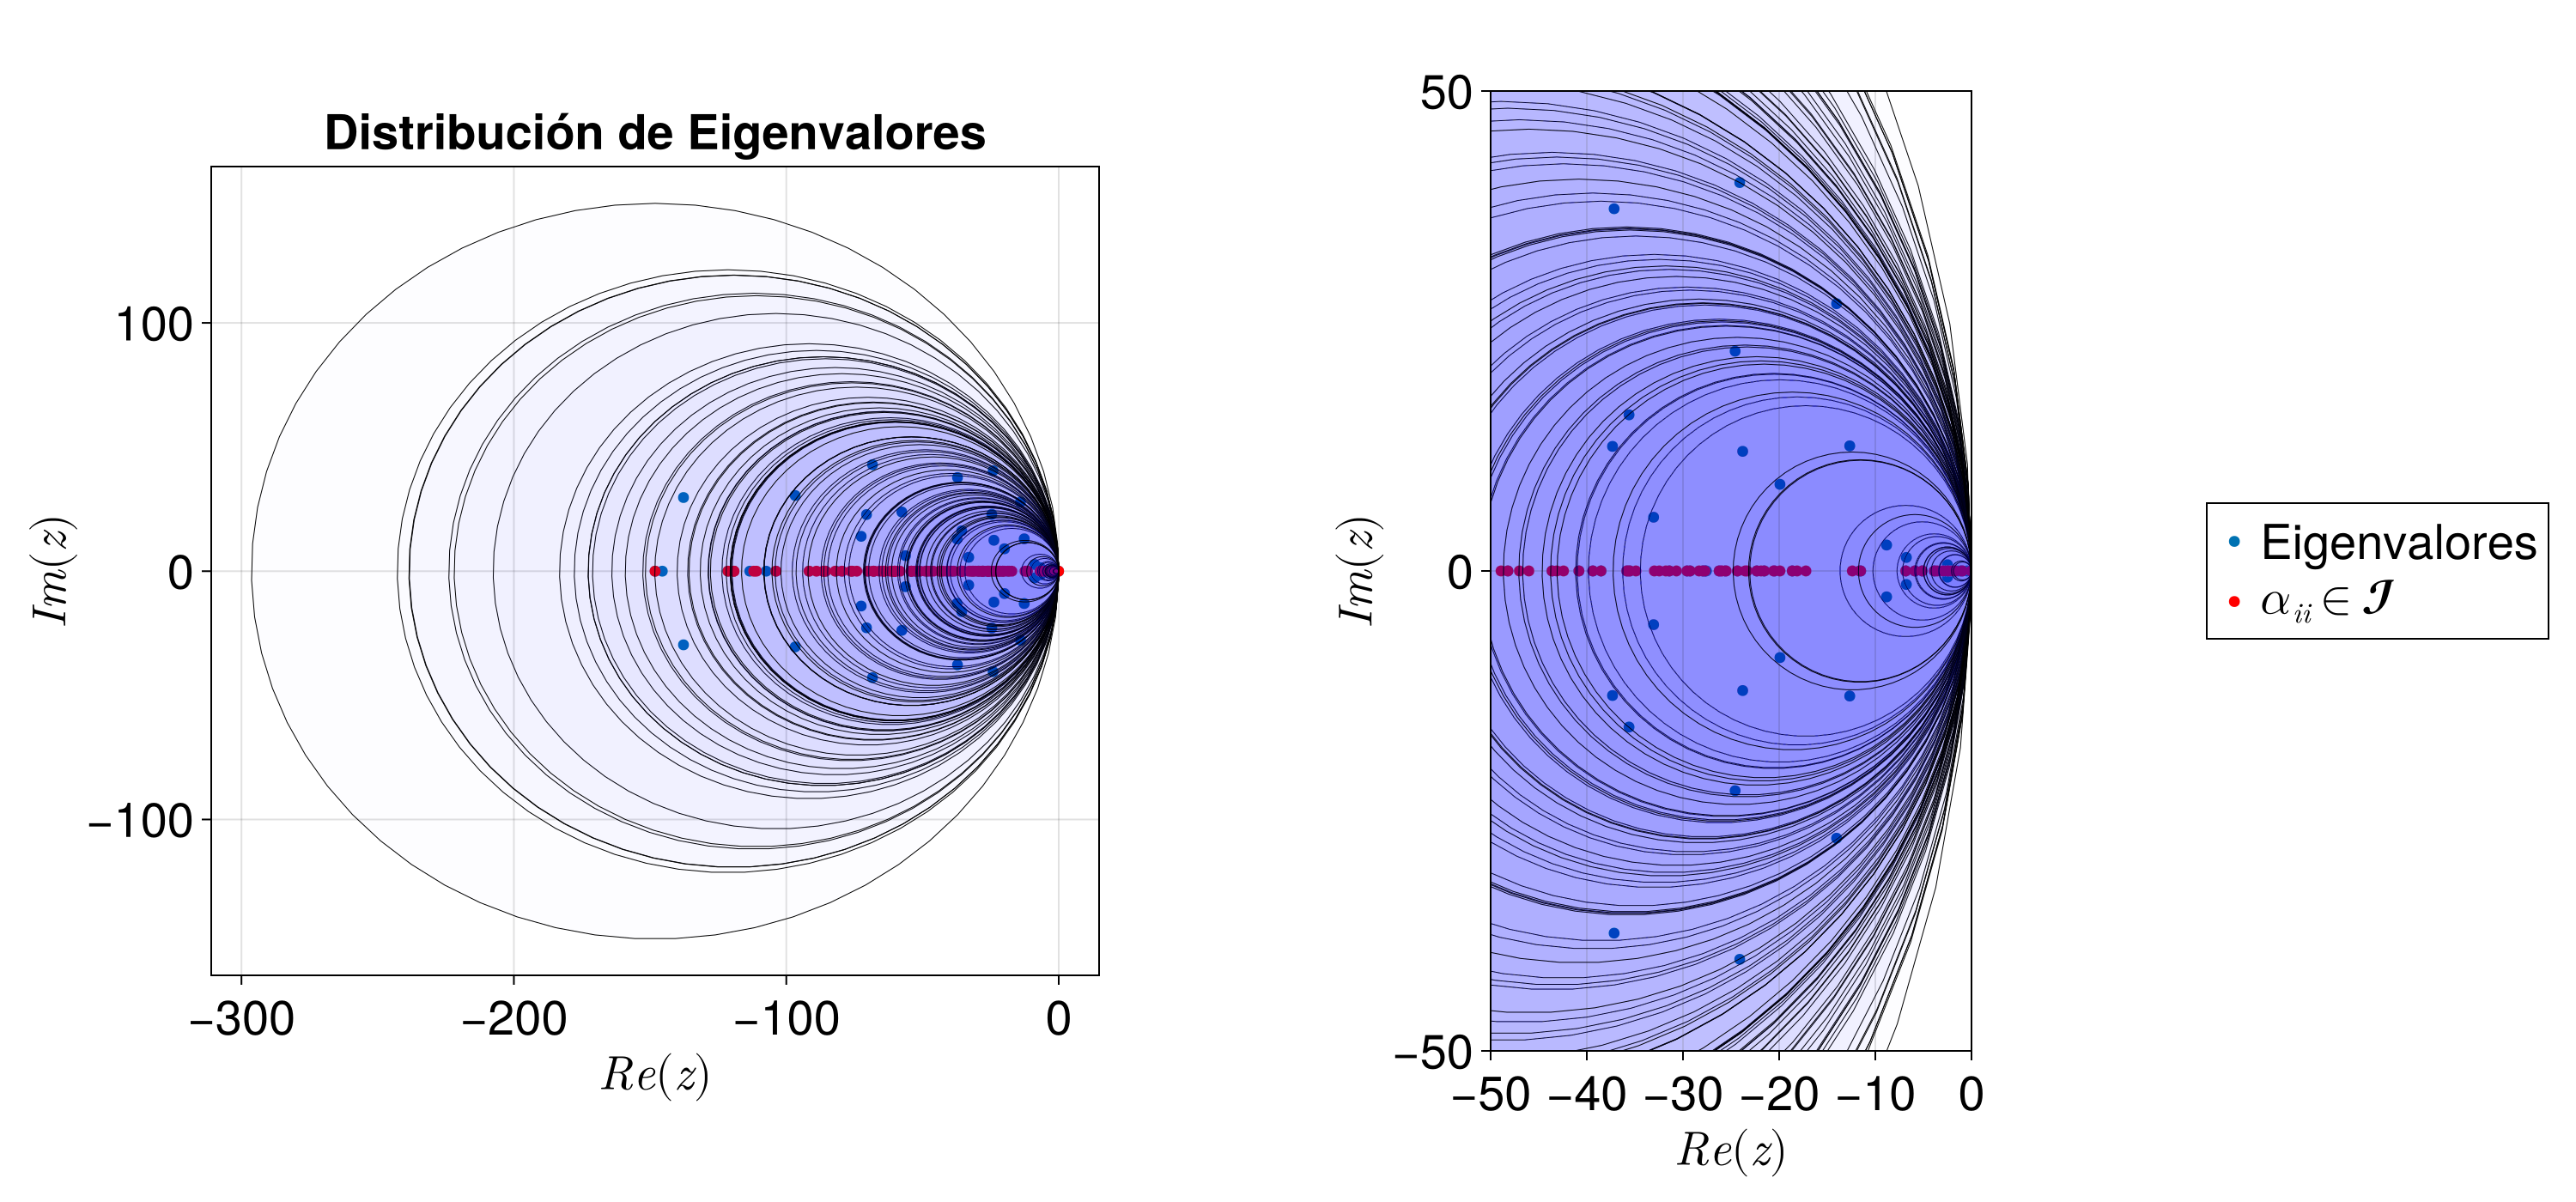
\includegraphics[scale=0.17]{../Imagenes/LeyesCirculares}
	\caption{Distribución de valores propios del sistema generalizado para $N=100$, $\sigma=0.2$ y $p=0.6$. Se consideran $N$ Leyes Circulares cuyo centro y radio es cada valor de la diagonal de la matriz Jacobiana asociada. }
	\label{fig:LeyesCirculares}
\end{figure}


\begin{wrapfigure}{l}{0.5 \textwidth} \vspace{-40pt} \begin{center}
	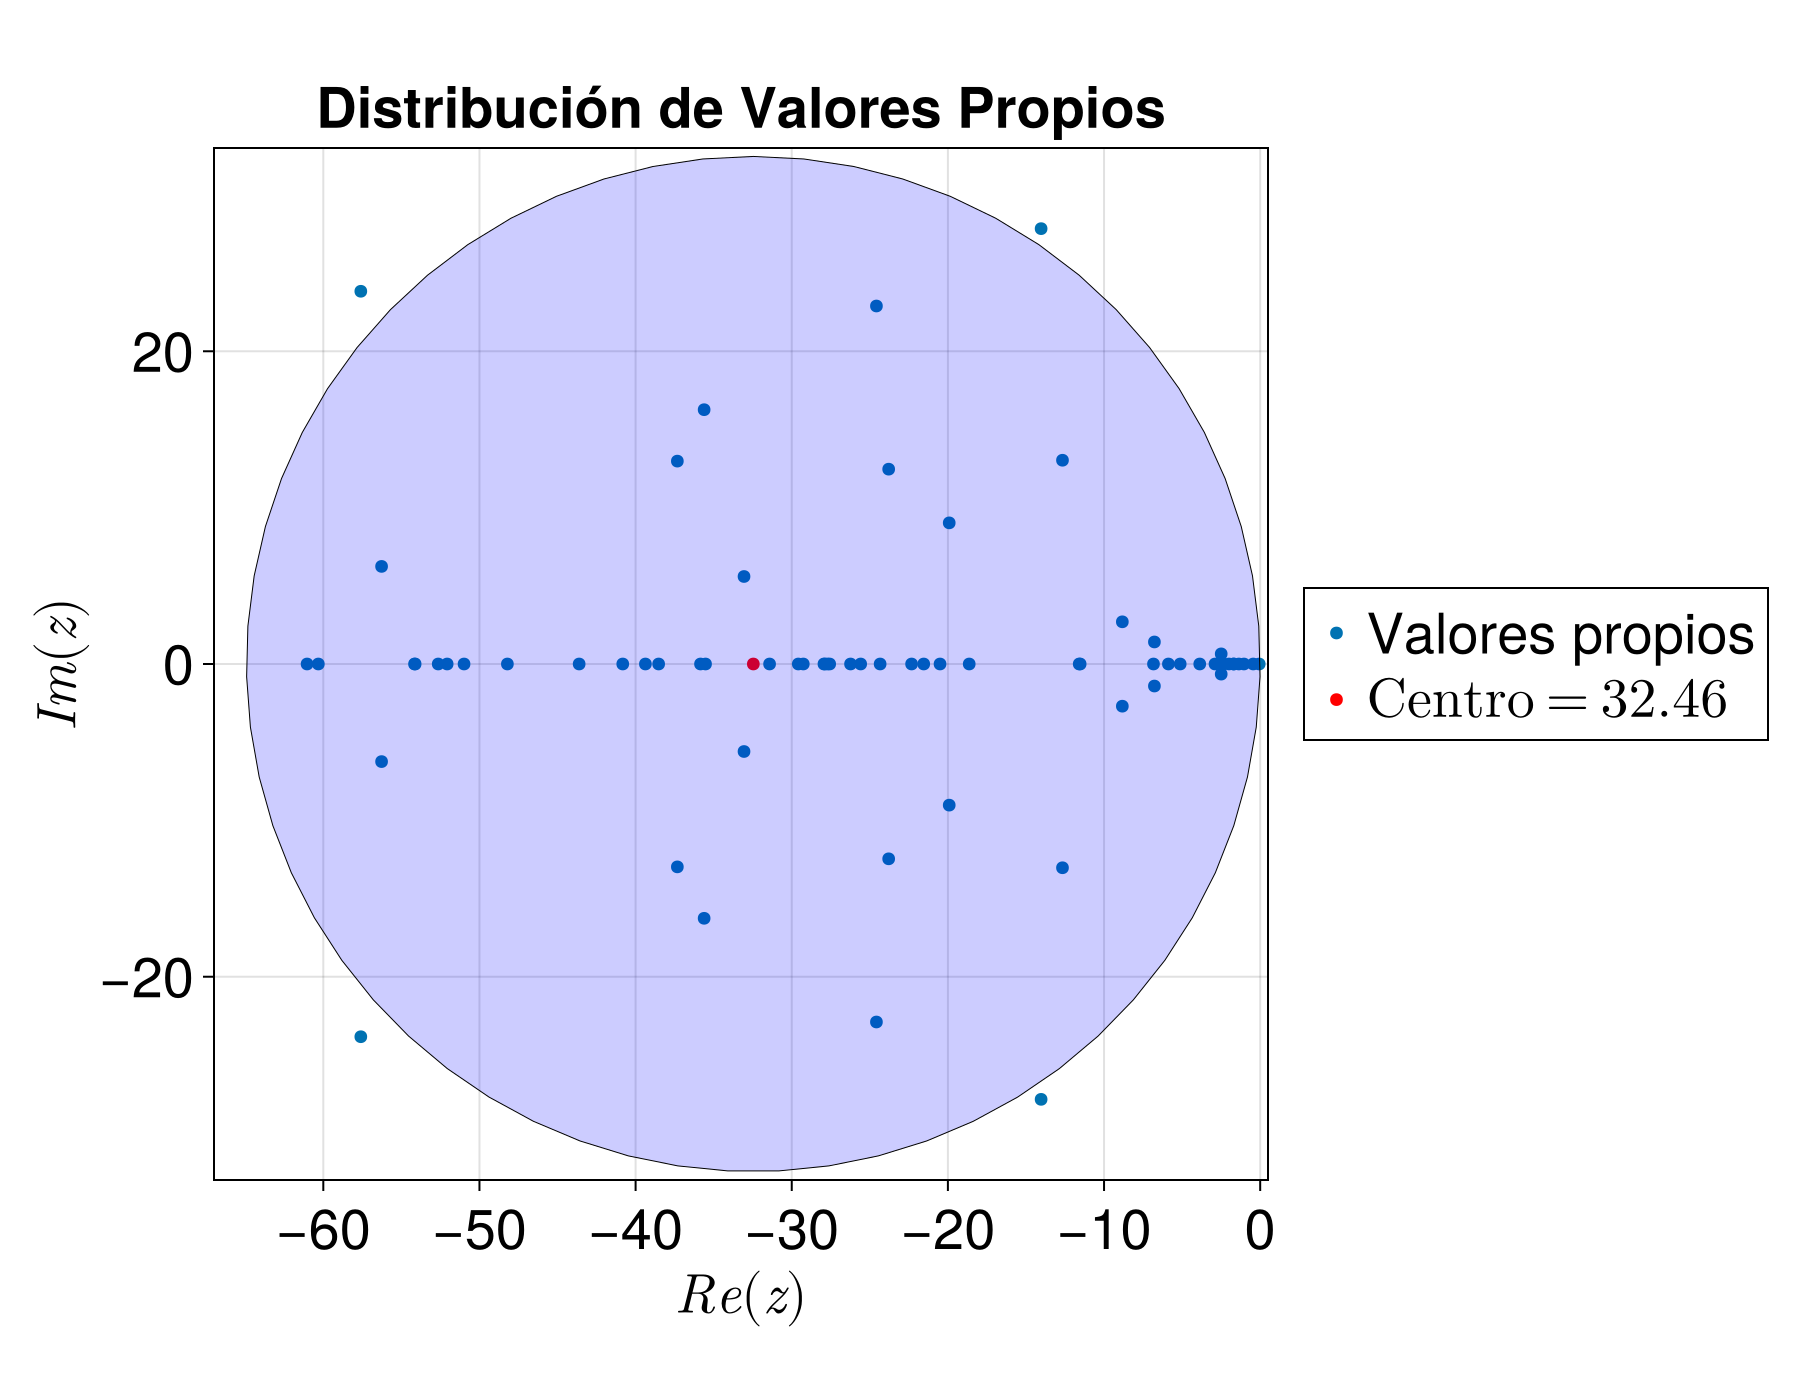
\includegraphics[scale=0.13]{../Imagenes/LeyCircularParticular}
	\end{center}
	\vspace{-20pt} 
	\caption{Caso particular de la Figura (\ref{fig:LeyesCirculares}) para el valor de la diagonal $\alpha_{ii}=32.46\in\mathcal{J}$.}
		\vspace{-10pt}
	\label{fig:LeyCircularParticular}
\end{wrapfigure}
Esta propuesta se inspira de la Proposición \ref{prop:DiagonalI}, en donde se invocaron los discos de Gershgorin que se encuentran centrados en cada valor de la diagonal de $\mathcal{J}$ y se demuestra que los radios pueden ser menores o iguales a cada uno de estos valores. Al ser menores o iguales, la actual propuesta toma el máximo caso posible (es decir la igualdad) y por lo tanto cada círculo encerrará un porcentaje de valores propios que se encuentren en la vecindad alrededor de $\mathcal{J}_{ii}$ de mismo radio.\\
\\
Un caso particular de la Figura (\ref{fig:LeyesCirculares}) considerando $\mathcal{J}_{ii}=32.46$ se puede observar en la Figura (\ref{fig:LeyCircularParticular}), cierto porcentaje de valores propios se distribuye por el círculo varios concentrados en el eje real solamente, sin embargo existen algunos otros que se escapan del confinamiento particular y pasan al siguiente nivel o círculo. Para poder confirmar o refutar esta propuesta, se explorarán múltiples sistemas estables con sus respectivas distribuciones de diagonales y valores propios.

\subsection{Análisis para $N=50$}

Se tienen a disposición dos conjuntos de datos, ambos son de simulaciones realizadas para diferentes valores de $p$ y $\sigma$. Cada conjunto esta conformado por 78 archivos .csv y son simulaciones de matrices \href{https://github.com/rogve98/Tesis/tree/master/Notebooks/Datos/Jacobianos}{Jacobianas} y de distribuciones de \href{https://github.com/rogve98/Tesis/tree/master/Notebooks/Datos/Diagonales}{Diagonales}\footnote{Para los Jacobianos acceder a: \url{https://github.com/rogve98/Tesis/tree/master/Notebooks/Datos/Jacobianos}. Para las Diagonales acceder a \url{https://github.com/rogve98/Tesis/tree/master/Notebooks/Datos/Diagonales}.}. Así mismo, en cada archivo se encuentran 100 simulaciones que resultaron estables y de los cuales se realizará el análisis correspondiente a la relación entre la distribución de las diagonales y de las partes reales de los valores propios de las matrices Jacobianas. En la siguiente tabla se muestra el esquema de simulaciones para cada $p$ y $\sigma$
\begin{table}[h!]
	\centering
	\begin{tabular}{|c|c|c|c|}
		\hline
		Fuerza promedio [$\sigma$] & Probabilidades [$p$] & Cantidad de archivos & Simulaciones realizadas \\ \hline
		$0.1-0.5$  & $0.1-1.0$  & 50 & 5000  \\ \hline
		0.6  & $0.1-0.9$  & 9 & 900 \\ \hline
		0.7  & $0.1-0.7$  & 7 & 700 \\ \hline
		0.8  & $0.1-0.5$  & 5 & 500 \\ \hline
		0.9  & $0.1-0.4$  & 4 & 400 \\ \hline
		1.0  & $0.1-0.3$  & 3 & 300 \\ \hline
		& \textbf{Total:} & 78& 7800\\ \hline
	\end{tabular}
	\caption{Cantidad de archivos generados para el banco de Diagonales y Jacobianos considerando $N=50$. A partir de $\sigma=0.6$ en adelante, los tiempos de compilación fueron muy prolongados por lo que no se obtuvieron los 10 archivos respectivos a diferencia de los valores promedio anteriores.}
	\label{tab:Simulaciones}
\end{table} 

La razón principal de escoger los sistemas para $N=50$ es por el costo computacional. Ha resultado muy prolongado el tiempo de compilación de sistemas más grandes (como el de $N=100$) y aún así para valores altos de la fuerza promedio ($\sigma\geq 0.6$) no se obtuvieron los 10 archivos por la misma razón. Habiendo introducido la información experimental, se procede a continuar con el análisis de las $N$ Leyes Circulares. Para ello convendrá determinar la correlación entre estas cantidades así como apreciar una comparativa visual entre la parte real y los valores de la diagonal.
\newpage
\begin{figure}[h!]
	\centering
	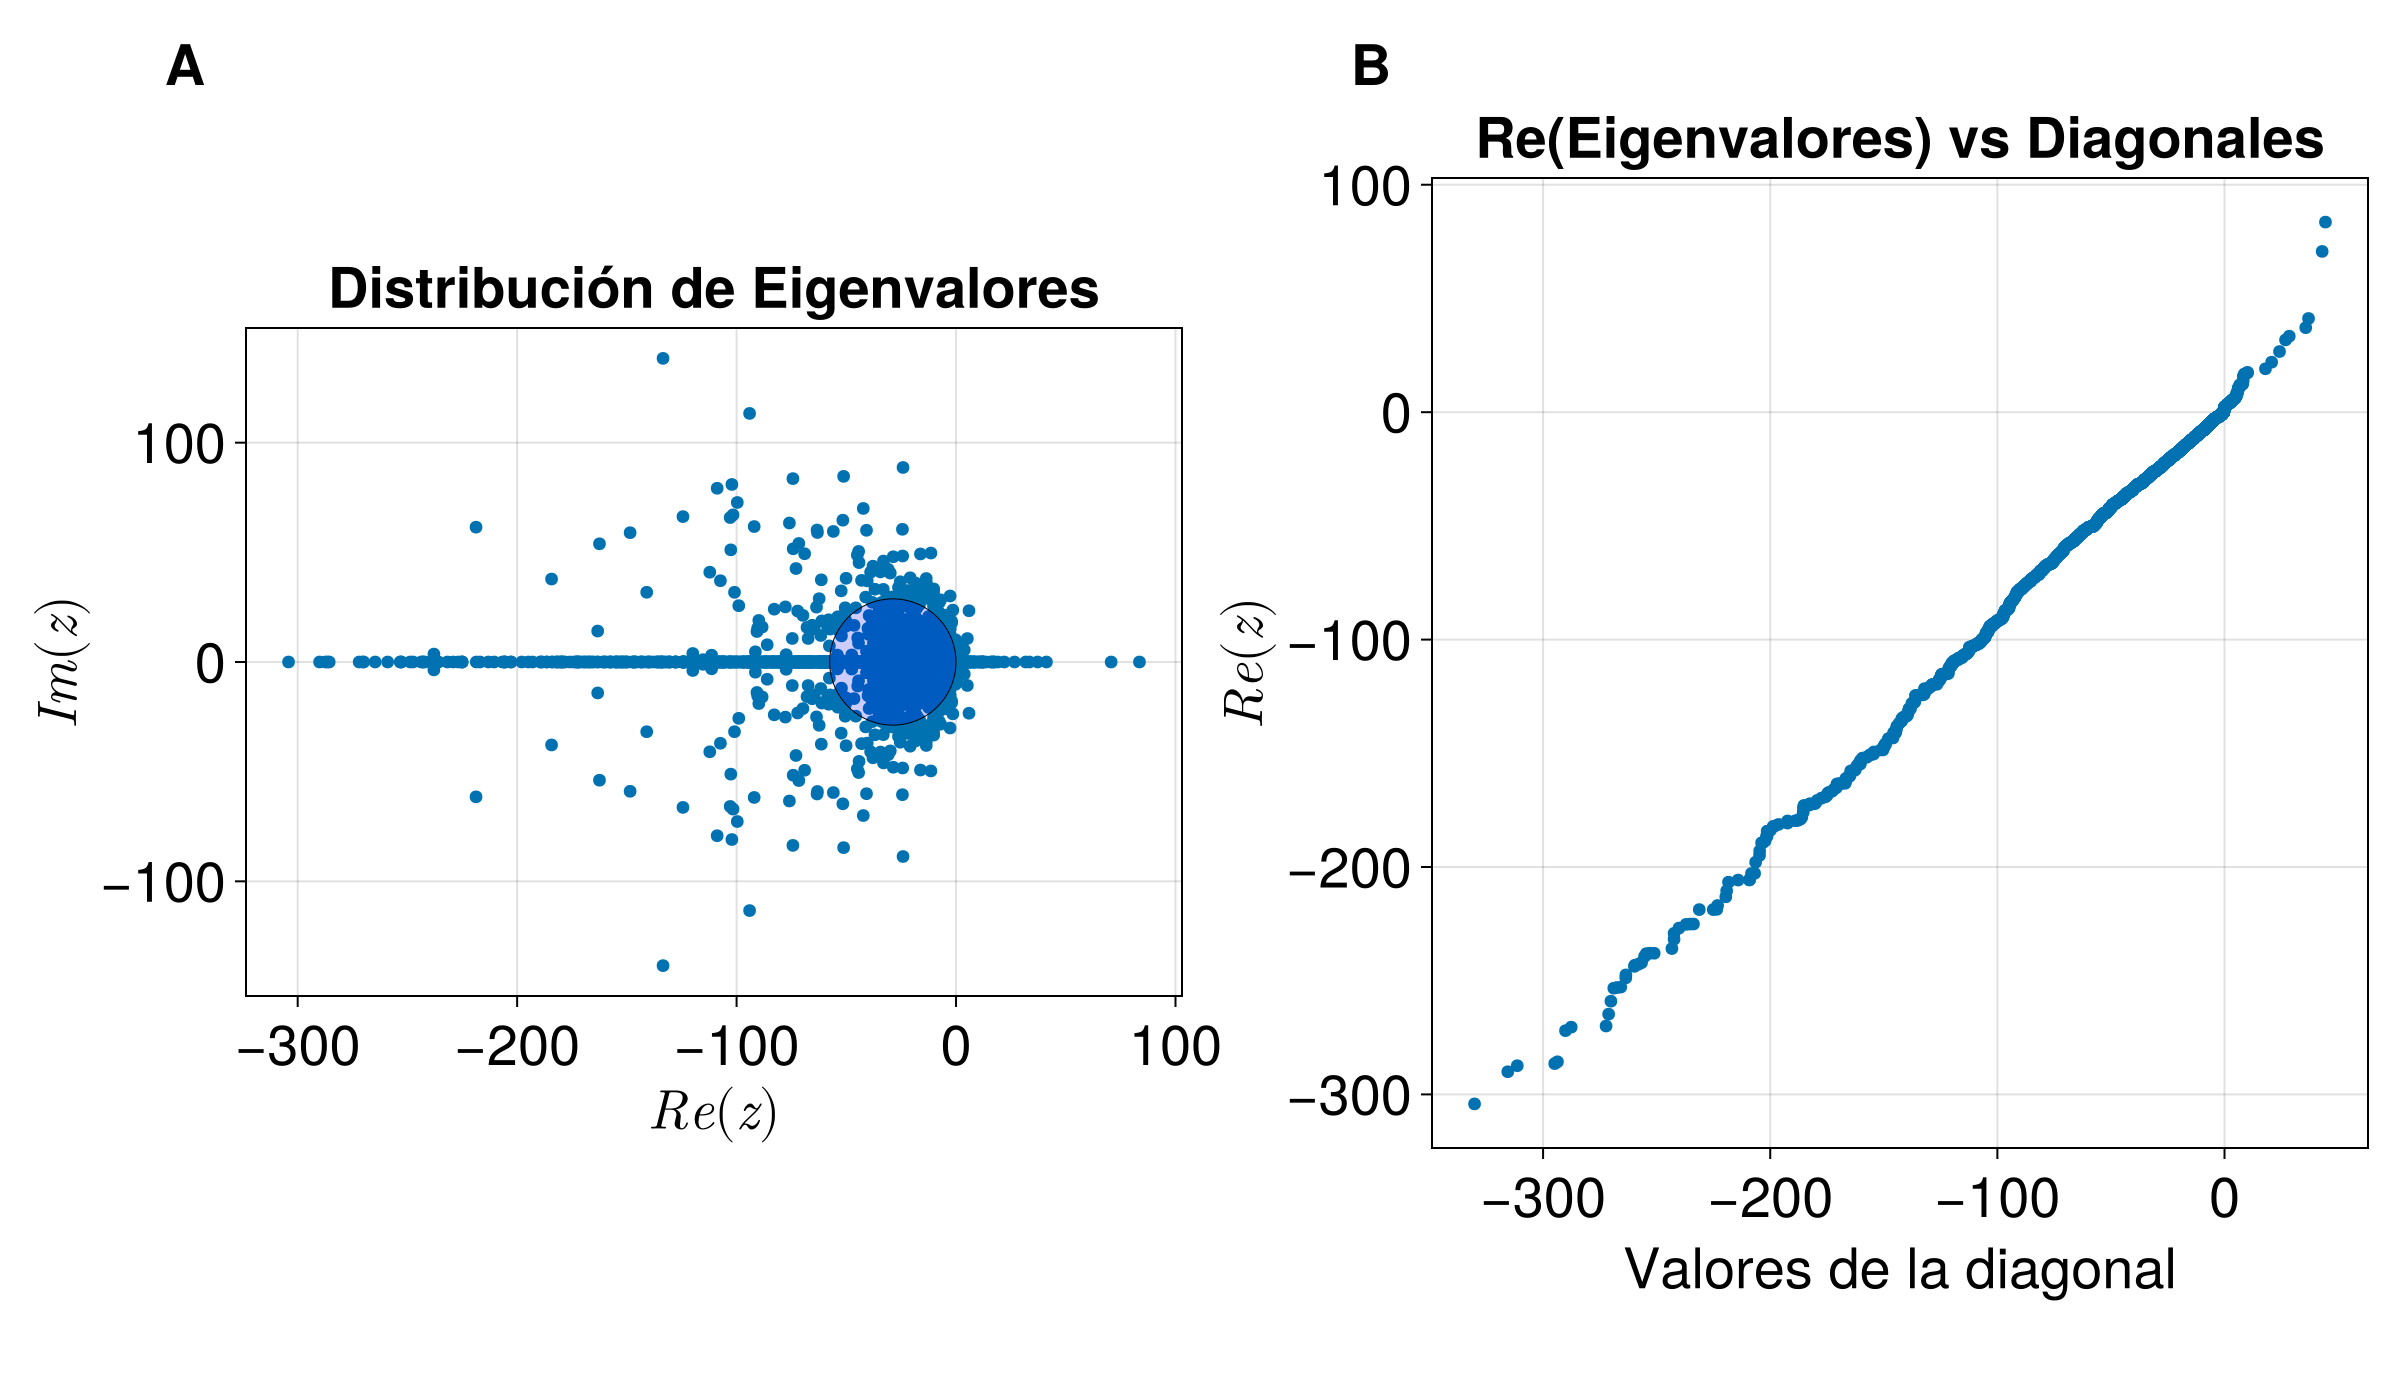
\includegraphics[scale=0.2]{../Imagenes/ReEvs-Diagonales}
	\caption{(\textbf{A}) Distribución de valores propios de 100 jacobianos para el caso $\sigma=0.5$, $p=0.5$. Se agrega una ley circular correspondiente al valor medio de la distribución de diagonales. (\textbf{B}) Relación entre la parte real de los valores propios con las diagonales de los Jacobianos considerados.}
	\label{fig:ReEvs-Diagonales}
\end{figure}

A simple vista se puede observar una relación lineal, y puede ser casi perfecta en algunos casos pero será cuestión de coincidencia, pues los valores propios se encuentran en las vecindades de Gershgorin alrededor de cada entrada de la diagonal de $\mathcal{J}$. Lo que nos muestra la Figura (\ref{fig:ReEvs-Diagonales} \textbf{B}) es que los $|\mathcal{J}_{ii}|$ más grandes de la distribución tienen un rango amplio en el radio de Gershgorin para alojar valores propios, lo que implica que posiblemente la parte real de de estos no se encuentre cerca de dicho valor $\mathcal{J}_{ii}$ y que por lo tanto no exista una relación tan lineal en estos casos.  A diferencia de los $|\mathcal{J}_{ii}|$ de menor tamaño que parecen tener un radio de Gershgorin proporcional y que ello implique que los valores propios se alojen cerca de dicho centro $\mathcal{J}_{ii}$ pudiendo marcar una mejor relación lineal. Más adelante se mostrará un ejemplo más evidente de este hecho.\\
\\
En la Figura (\ref{fig:ReEvs-Diagonales} \textbf{A}) se ha agregado una Ley Circular particular con centro y radio correspondiente al valor medio de la distribución, esto con el fin de observar que tan significativa es la media de la distribución en cuanto a ver cuantos valores propios es capaz de encerrar. Aunque encierra una gran cantidad de ellos, también un gran porcentaje queda fuera por lo que la media no es un valor representativo de la distribución en este caso. Para seguir explorando si la relación lineal existe también para el resto de las simulaciones de la Tabla (\ref{tab:Simulaciones}) se tomará la media, mediana y moda de las distribuciones de diagonales $d(\sigma_i,p_j)$ y partes reales de los conjuntos de valores propios $\overline{\lambda}$ para compararlos viendo si existe una correspondencia lineal entre estas cantidades.
\begin{figure}[h!]
	\centering
	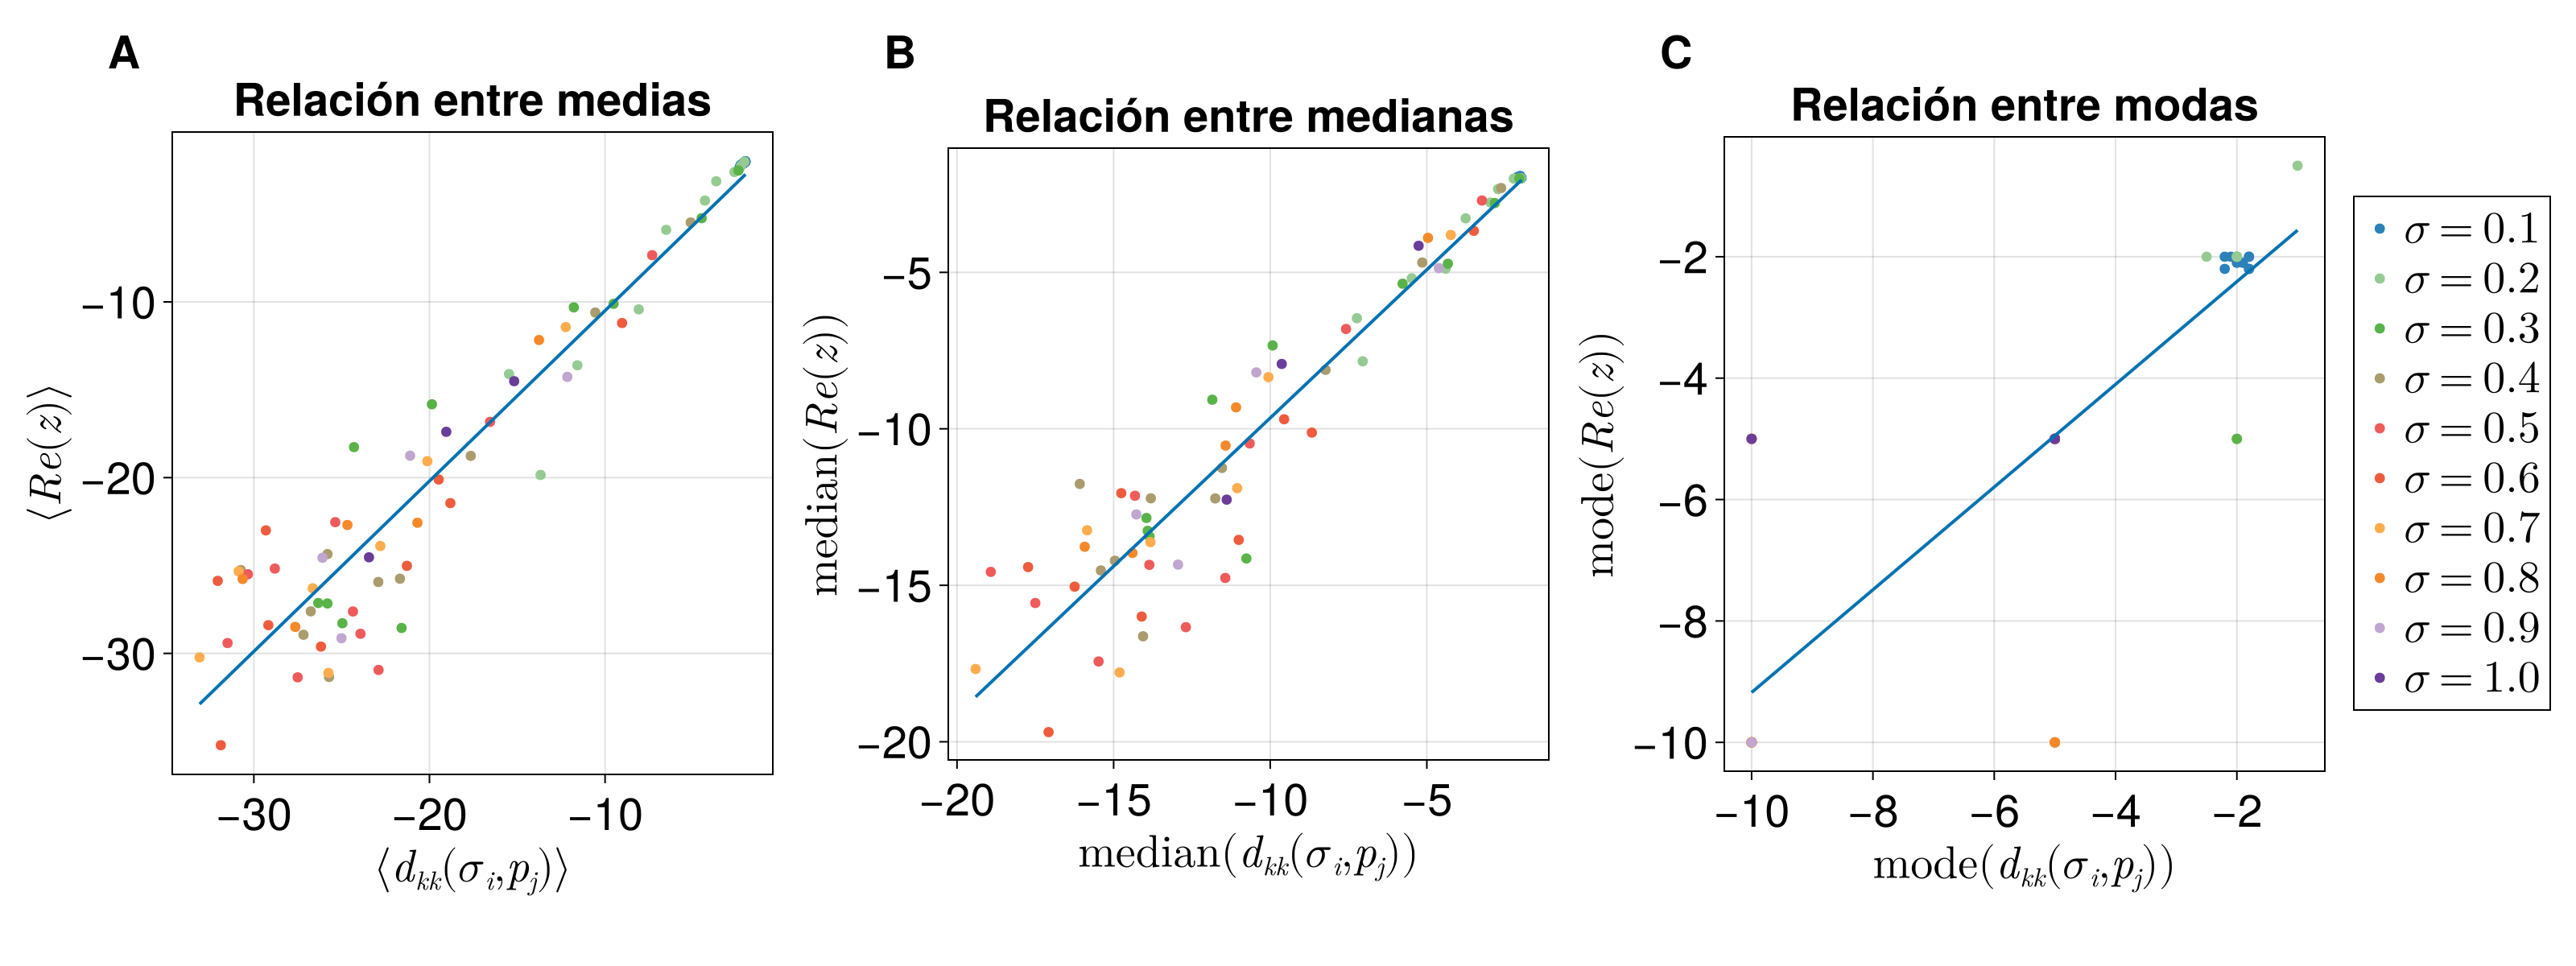
\includegraphics[scale=0.16]{../Imagenes/AjustesLinMeds}
	\caption{(\textbf{A}) Ajuste lineal de la relación entre las medias de las $Re(\overline{\lambda})$ con las medias de las $d(\sigma_i,p_j)$ de las Jacobianas del sistema. (\textbf{B}) Ajuste lineal de la relación entre las medianas $Re(\overline{\lambda})$ con las medianas de las $d(\sigma_i,p_j))$ de las Jacobianas del sistema. (\textbf{C}) Ajuste lineal de la relación entre las modas de $Re(\overline{\lambda})$ con las modas de las $d(\sigma_i,p_j)$ de los Jacobianas del sistema.}
	\label{fig:AjustesLinMeds}
\end{figure}

En la Figura (\ref{fig:AjustesLinMeds}) se distingue la media, mediana y moda de cada distribución; cada color se encuentra asociado a los valores de la fuerza promedio $\sigma$ y la cantidad de puntos del mismo color corresponde a cada una de las probabilidades de conectividad del sistema. Se ha visto en la Figuras (\ref{fig:DistDiagonal}, \ref{fig:DistEigenvalores}) que cuando esta probabilidad es cada vez mayor entonces las colas de sus distribuciones son cada vez más anchas debido a la posibilidad de mayor cantidad de interacciones y la dependencia que hay con los valores del punto fijo del sistema. Por lo tanto hacia la izquierda estarán las probabilidades más grandes e irán decreciendo hacia la derecha.\\
\\
En cada gráfica de esta figura se encuentran las 78 simulaciones realizadas y se nota claramente una correspondencia entre los valores de la diagonal con las partes reales de los valores propios, lo que refuerza la propuesta de las Leyes Circulares antes mencionada. Al igual que en la Figura (\ref{fig:ReEvs-Diagonales}), cada ajuste es mejor para valores cercanos al cero que para los máximos en valor absoluto, esto debido al argumento antes mencionado sobre la amplitud del radio de Gershgorin que implica que los valores propios tengan la posibilidad de alojarse lejos del correspondiente centro $\mathcal{J}_{ii}$.\\
\\
Lo que se pudo observar de estas revisiones es que ambas distribuciones siguen una tendencia de distribución de cola pesada con sesgo negativo hacia la derecha. Una hipótesis por comprobar y que se escapa de los objetivos de esta tesis, sería investigar si la distribución de las entradas del punto fijo estable asociadas a las matrices Jacobianas de los sistemas impacta directamente en como son las distribuciones de las diagonales y a su vez las de las partes reales de los valores propios. Para tener mayor certeza de la relación lineal, se presentará la correlación que existen entre ambas distribuciones.	
\begin{figure}[h!]
	\centering
	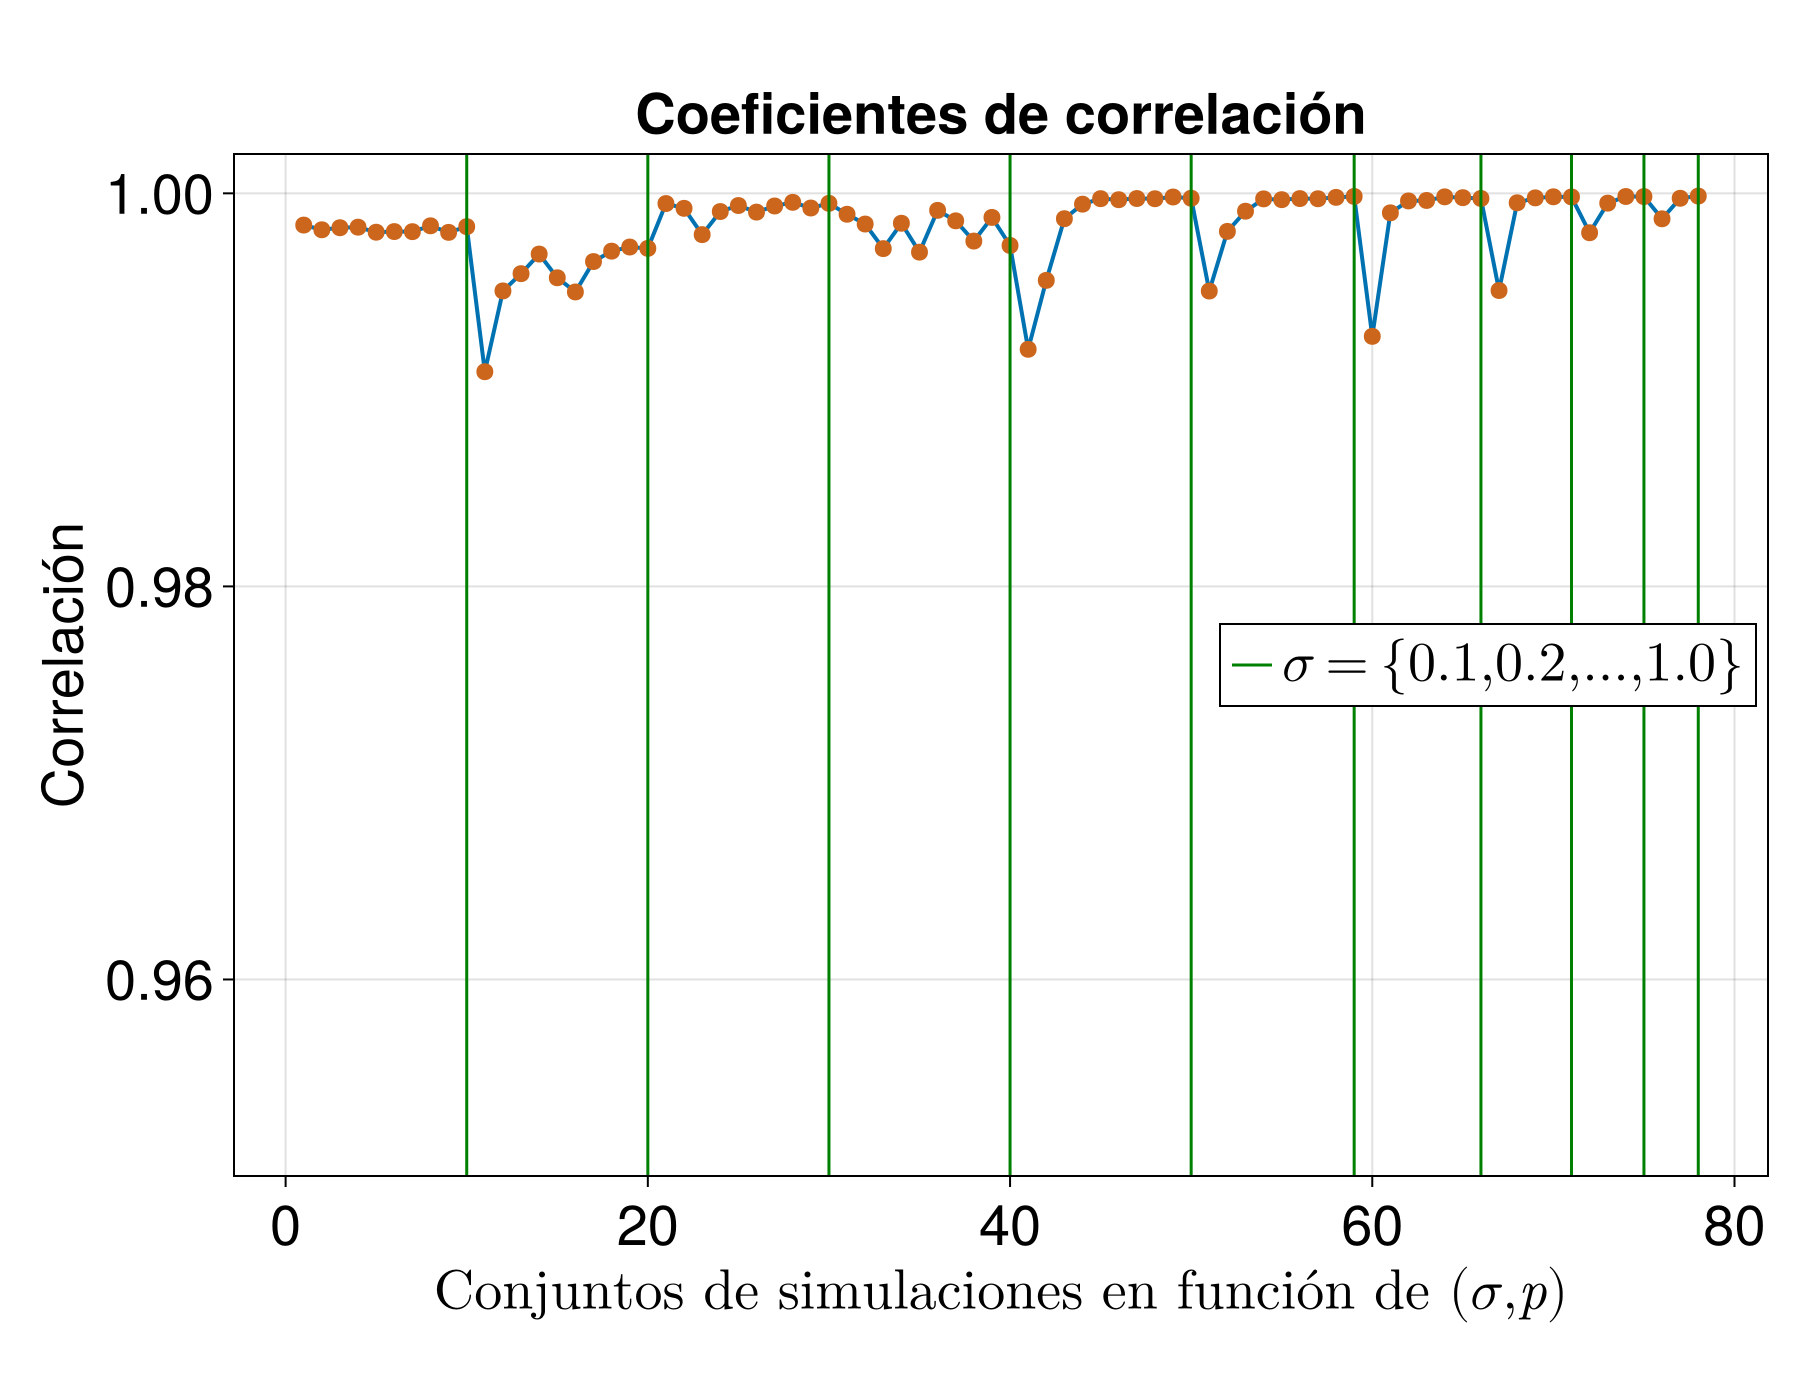
\includegraphics[scale=0.2]{../Imagenes/CoeficientesCorrelacionN}
	\caption{Coeficientes de correlación en función de $\sigma$ y $p$. Cada uno de los 78 coeficientes corresponde para un conjunto $\sigma_i$ y $p_j$ de simulaciones según la Tabla (\ref{tab:Simulaciones}).}
	\label{fig:CoeficientesCorrelacionN}
\end{figure}

Esta muestra contiene un coeficiente de correlación por cada simulación realizada. Para determinar cada uno de ellos se consideró cada distribución, tanto de diagonales como de partes reales de los valores propios. Cada línea verde delimita un conjunto de simulaciones por cada $\sigma$ de acuerdo con la 
\begin{wrapfigure}{r}{0.5 \textwidth} \vspace{-30pt} \begin{center}
		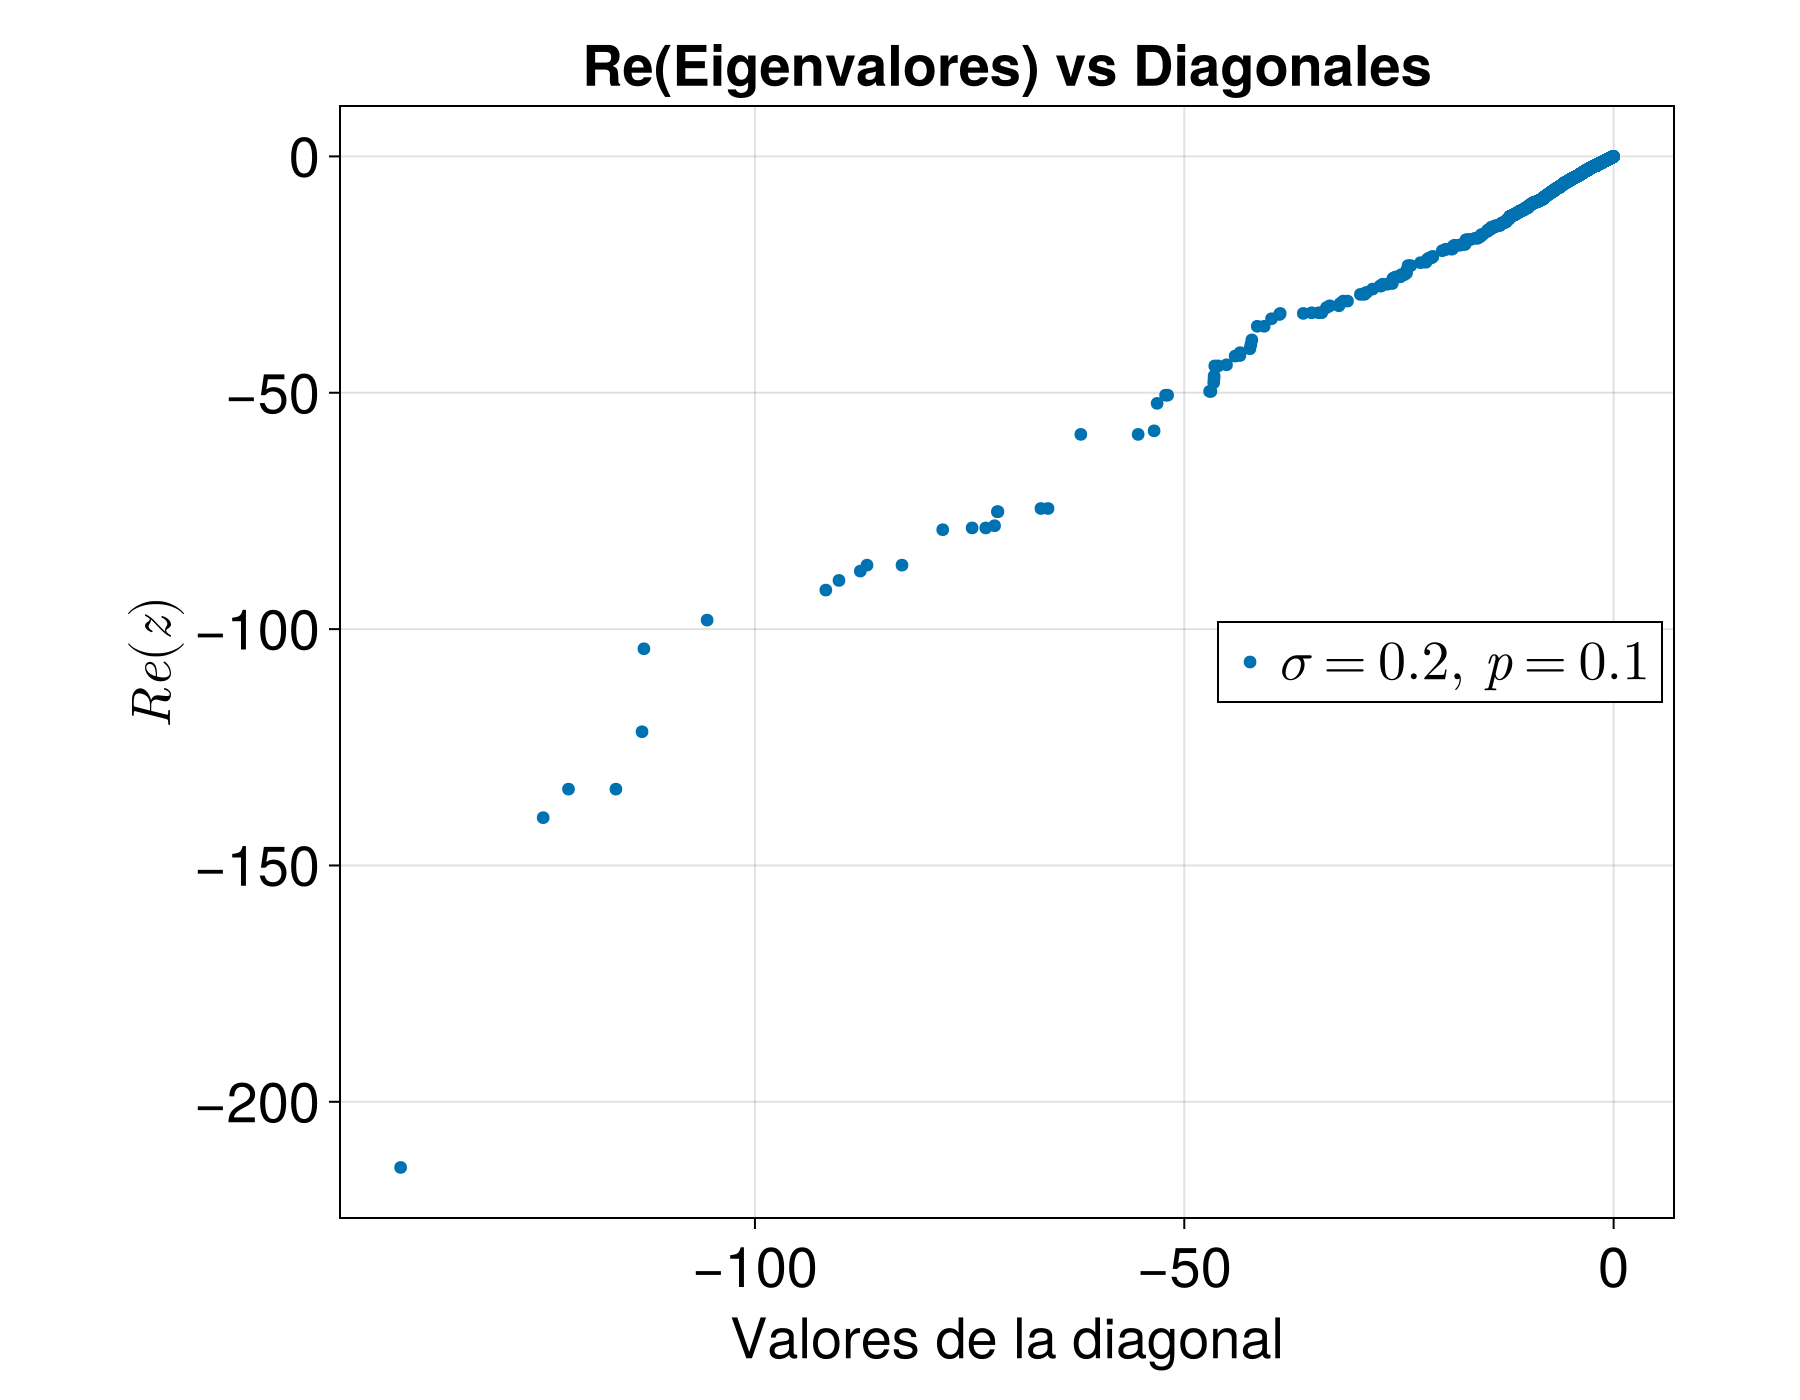
\includegraphics[scale=0.135]{../Imagenes/AnomaliaSim11}
	\end{center}
	\vspace{-20pt} 
	\caption{Relación entre cantidades de la simulación 11, caso con $\sigma=0.2$ y $p=0.1$.}
	\vspace{-10pt}
	\label{fig:AnomaliaSim11}
\end{wrapfigure}
Tabla (\ref{tab:Simulaciones}). En general se puede apreciar una correlación casi perfecta en entre las distribuciones consideradas, lo que implica que si existe una dependencia en la forma de la distribución de valores propios en función de las entradas de las diagonales. Así mismo, sustenta la propuesta de las Leyes Circulares, pues cada elemento de las diagonales esta íntimamente relacionado con al menos un valor propio de su respectiva matriz Jacobiana. Este diagrama puede servir para tener un mapa general de como es la relación entre distribuciones, se puede observar un caso excepcional para los valores $\sigma=0.2$ y $p=0.1$, en este caso aunque la correlación sigue siendo muy alta, es la menor de todo el conjunto de simulaciones. Viendo la Figura (\ref{fig:AnomaliaSim11}) se puede notar que son los máximos en valor absoluto los que tienen discrepancias a tal nivel que rompe con la linealidad.

\section{Transiciones de estabilidad}

Para darle seguimiento a los resultados de esta tesis, esta sección se va a centrar en explorar de forma cualitativa las condiciones de estabilidad de los sistemas de Lotka-Volterra generalizado en función de $\sigma$ y $p$. Posteriormente se presentará un análisis sobre las condiciones de la matriz de incidencias para que exista o no estabilidad en los sistemas relacionados, con miras en presentar un primer esbozo del parámetro crítico de transición que resulta no ser trivial de hallar. Para el caso más robusto ($N=100$) se va a presentar la diferencia entre usar matrices estructuralmente simétricas y puramente aleatorias (como el caso de May), reforzando el hecho de que la simetría entre interacciones presentan elementos adicionales que determinan la estabilidad, tal y como se vio al final del capítulo anterior.\\
\\
Se van a considerar tres tipos de sistemas, para $N=\{100,50,25\}$. Se pretende ver como cambia la estabilidad con diferentes tamaños del sistema (\ref{eqn:LK}). El proceso para llevar a cabo la construcción de los diagramas de transición es semejante al que se presentó en la sección de las Transiciones de May, se va a integrar el sistema fijando la fuerza de interacción en los siguientes valores ${\Sigma}=\{0.1,0.2,...,1.0\}$ mientras que para las probabilidades de conectividad se va a considerar la siguiente partición del intervalo $[0,1]$ para cada $N$:
\begin{equation}\label{eqn:particionLin}
	p = \{x_i\, |\, x_i=i\cdot\Delta x, i=0,1,2,...,100\},\qquad\text{con }\Delta x=0.01
\end{equation}
Con esta configuración de valores se permitirá generar diagramas de estabilidad para cada $N$ en función de $p$ considerando que es una partición equidistante. Hay otros dos diagramas de estabilidad que son de interés; siguiendo en función de la probabilidad de conectividad se define la siguiente partición sobre el intervalo $[0,1]$
\begin{equation}\label{eqn:particionLog}
	p_{\log}=\left \{ x_i\, |\, x_i=10^{-\left (10-\frac{10i}{99}\right )},\ i=0,1,...,99\right \}
\end{equation}
Se ha considerado particularmente este conjunto de probabilidades ya que para ciertas $\sigma\in\Sigma$ y para $N=100$ primordialmente, la transición ocurre de manera abrupta de modo que no se aprecia con claridad cuando ocurre. Por este motivo se utiliza esta escala de valores para poder visualizar los cambios para probabilidades muy pequeñas. Por último pero no menos importante, se van a considerar diagramas en donde se deja fija la $p$ para cada $N$ y se define una partición equidistante en el intervalo $[0,1]$ en función de la fuerza de interacción, es decir:
\begin{equation}\label{eqn:particionSigma}
	\sigma = \{x_i\, |\, x_i=i\cdot\Delta x, i=0,1,2,...,100\},\qquad\text{con }\Delta x=0.01
\end{equation}
Para esta configuración de valores se obtendrán los diagramas de transición en función de $\sigma$ y se verá que tan contrastante es con respecto de los otros diagramas de transición; se verá que sigue la tendencia de las transiciones de May, pues estas también ocurren más hacia la derecha que las que van en función de $p$. \\
\\
Teniendo las particiones y los ajustes de parámetros necesarios para generar los diagramas de transición, solamente falta ver cómo y de qué manera se van a generar estos diagramas. Se integrará el sistema cierto número de veces para cada $N$, $\sigma$ y $p$ con sus correspondientes particiones y por cada elemento de dicha partición:
\begin{table}[h!]
	\centering
	\begin{tabular}{|c|c|}
		\hline
		Tamaño del sistema $N$ & Cantidad de simulaciones por cada elemento de la partición  \\ \hline
		100 & 3000 \\ \hline
		50  & 6000 \\ \hline
		25  & 12000 \\ \hline		
 	\end{tabular}
	\caption{Cantidad de simulaciones realizadas por cada $N$ y para cada elemento de la partición definida.}
	\label{tab:SimulacionesTransicion}
\end{table} 

De tal forma que se van a determinar cuantos sistemas resultaron estables del total de simulaciones realizadas para dicho elemento y se contabilizarán. Se podrá percibir como un porcentaje de estabilidad y se podrá observar que cuando los valores de cada partición aumentan, la estabilidad de los sistemas irá decreciendo. La elección de la cantidad de simulaciones realizadas para cada conjunto de sistemas en función de $N$ responde a la intención de suavizar las curvas; entre más valores se consideren, la curva se hace cada vez más suave debido a la ley de los grandes números. Se ha observado que entre más chico sea el tamaño del sistema se requieren mas simulaciones para poder suavizar dicha curva.\\
\\
%En una primera versión de resultados se consideró un método que generó algunos problemas los cuales se visualizaron en la sección anterior, en la discusión de los sistemas asintótica-mente estables: los cuales no alcanzaron su estabilidad o quizás no eran estables y todo gracias al tiempo de integración de $t_f=50$. Sin embargo se han generado otros resultados en donde se pone una restricción para que solamente se consideren sistemas que se integren en un tiempo máximo de $t_f=50$. Entre ambos tipos de resultados existen algunas desviaciones que requerirán de su análisis más adelante. Habiendo conseguido los diagramas de transición mediante todo un proceso computacionalmente arduo, merece preguntarse si acaso estas transiciones  de estabilidad corresponden con transiciones de fase, y de ser cierto ¿cuál sería su parámetro crítico? Se tiene una pista en la relación (\ref{eqn:paramMay}) que re acomodando se tiene
%\begin{equation}\label{eqn:ParametroCritico}
%	\sigma\sqrt{NC}<d
%\end{equation}
%donde en el caso de May corresponde con la diagonal fijada en $-d=-1$. Se explorará si en los diagramas de transición generados existe alguna dependencia/relación con algún valor representativo de las $d_{kk}(\sigma_i,p_j)$ de los Jacobianos del sistema.
Retomando la discusión generada en el capítulo anterior derivada de la Proposición \ref{prop:paramMay}, se había concluido que el parámetro de transición de May (\ref{eqn:radioMayGirko}) no puede ajustarse directamente a las transiciones del sistema de Lotka-Volterra generalizado. La razón fundamental de ello se encuentra en la forma que tienen las matrices Jacobianas del Sistema de Lotka-Volterra generalizado. No cumplen la regla de tener entradas i.i.d. con media cero y varianza $\sigma^2$\footnote{Condición necesaria para la Ley Circular de Girko que justifica el resultado del parámetro de May (\ref{eqn:radioMayGirko}).}, sino que la diagonal tiene una forma de distribución de cola pesada y con sesgo negativo, y el resto de las entradas de la matriz no viene necesariamente de una distribución normal (Ver ec. (\ref{eqn:MartizJacobiana})).
\\
\\
Por lo tanto habrá que explorar otra alternativa para poder acercarse al parámetro de transición de éstos sistemas. Considerando adicionalmente el impacto de los puntos fijos y su distribución que induce a la forma de las matrices Jacobianas, no dejando atrás el papel que tiene la matriz de incidencias $\Lambda$ para a su vez inducir a estos puntos fijos. Finalmente considerar que $\Lambda$ es estructuralmente simétrica implicando más elementos que inciden en la estabilidad (Ver Fig. (\ref{fig:TransicionDirvsNoDir})).

\subsection{Para $N=100$}

\subsubsection*{En función de $p$}

Este sistema es el más robusto analizado y del que se le podría extraer más información debido a las características de sus diagramas de transición. Como bien se mencionó anteriormente, se necesitó una cantidad de simulaciones considerablemente inferior en comparación con los sistemas $N=50,25$ (Tabla (\ref{tab:SimulacionesTransicion})), lo que por sí mismo demuestra que la cantidad de interacciones esta relacionada con la ley de los grandes números, entre más grande sea el sistema: mayor será su capacidad de ``promediar'' el ruido estocástico interno y por lo tanto sus fluctuaciones irán disminuyendo permitiendo que el promedio converja cada vez mejor al valor esperado.
\begin{figure}[h!]
	\centering
	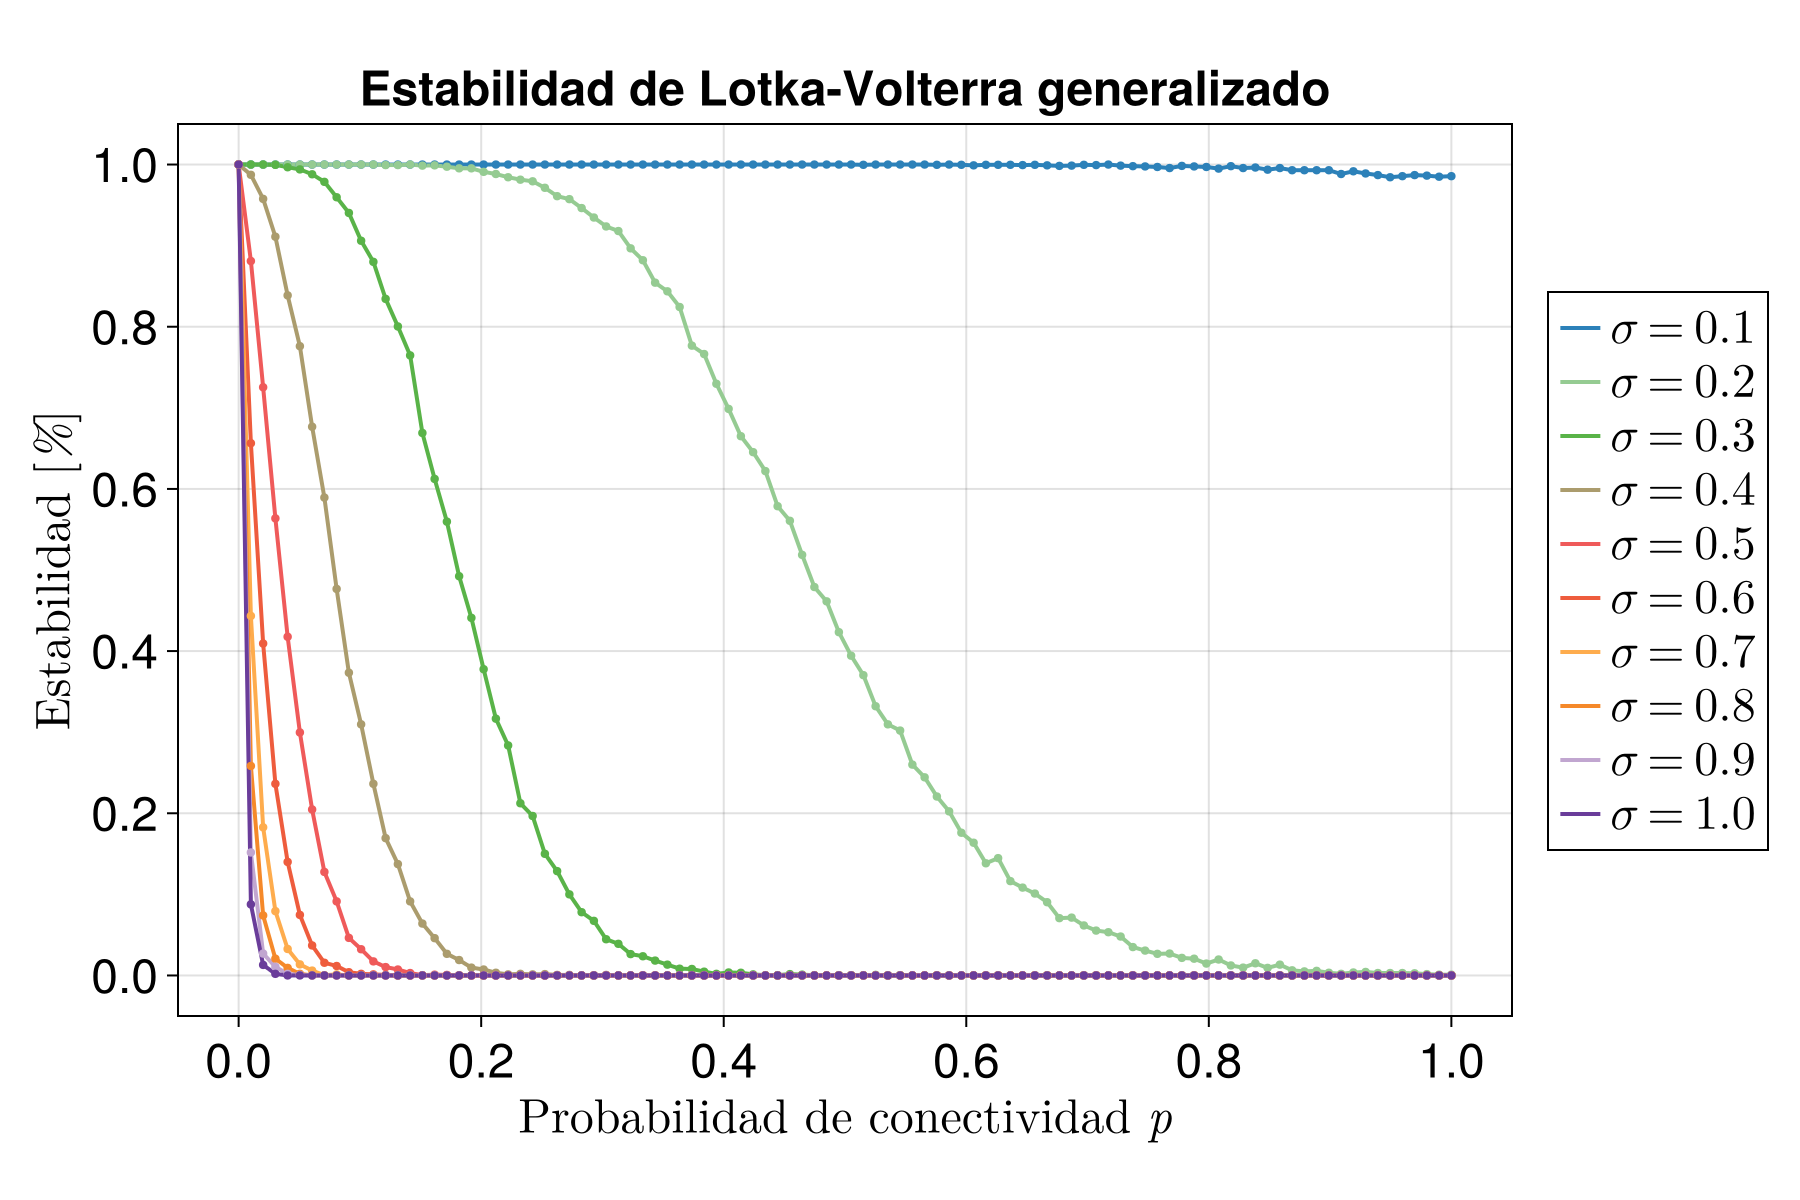
\includegraphics[scale=0.2]{../Imagenes/EstabilidadLKpLin.png}
	\caption{Transiciones de estabilidad en el Sistema de Lotka-Votlerra generalizado en función de la probabilidad de conectividad para $N=100$.}
	\label{fig:EstabilidadLKpLin}
\end{figure}

En este diagrama al igual que en el May (Fig. \ref{fig:TransicionMayDirLin}) también se observa un cambio abrupto para $\sigma>0.3$ ubicado en los primeros valores de la probabilidad, sin embargo, su diferencia radica en la suavidad con la que ocurren en el Sistema de Lotka-Volterra generalizado. Una suavidad muy semejante a la que presentan los sistemas de May que son estructuralmente simétricos, sobre todo mucho más marcadas para los valores de $\sigma$ cercanos a 1. \\
\\
En este caso se abre el análisis con matrices de incidencias $\Lambda$ estructuralmente simétricas que dan origen a Jacobianas de la misma naturaleza, más adelante se realizará una comparación (únicamente para el caso $N=100$) entre sistemas con interacciones aleatorias y estructuralmente simétricas.
\newpage
Nuevamente se ajusta el eje $x$ en escala logarítmica para lograr visualizar las transiciones con $\sigma>0.3$. Se puede observar que aún para valores de $\sigma$ cercanos a 1, sigue presentando una notoria suavidad con respecto de los sistemas de May (Fig. \ref{fig:TransicionMayDirLog}) que son sustancialmente similares a los sistemas de May estructuralmente simétricos.
\begin{figure}[h!]
	\centering
	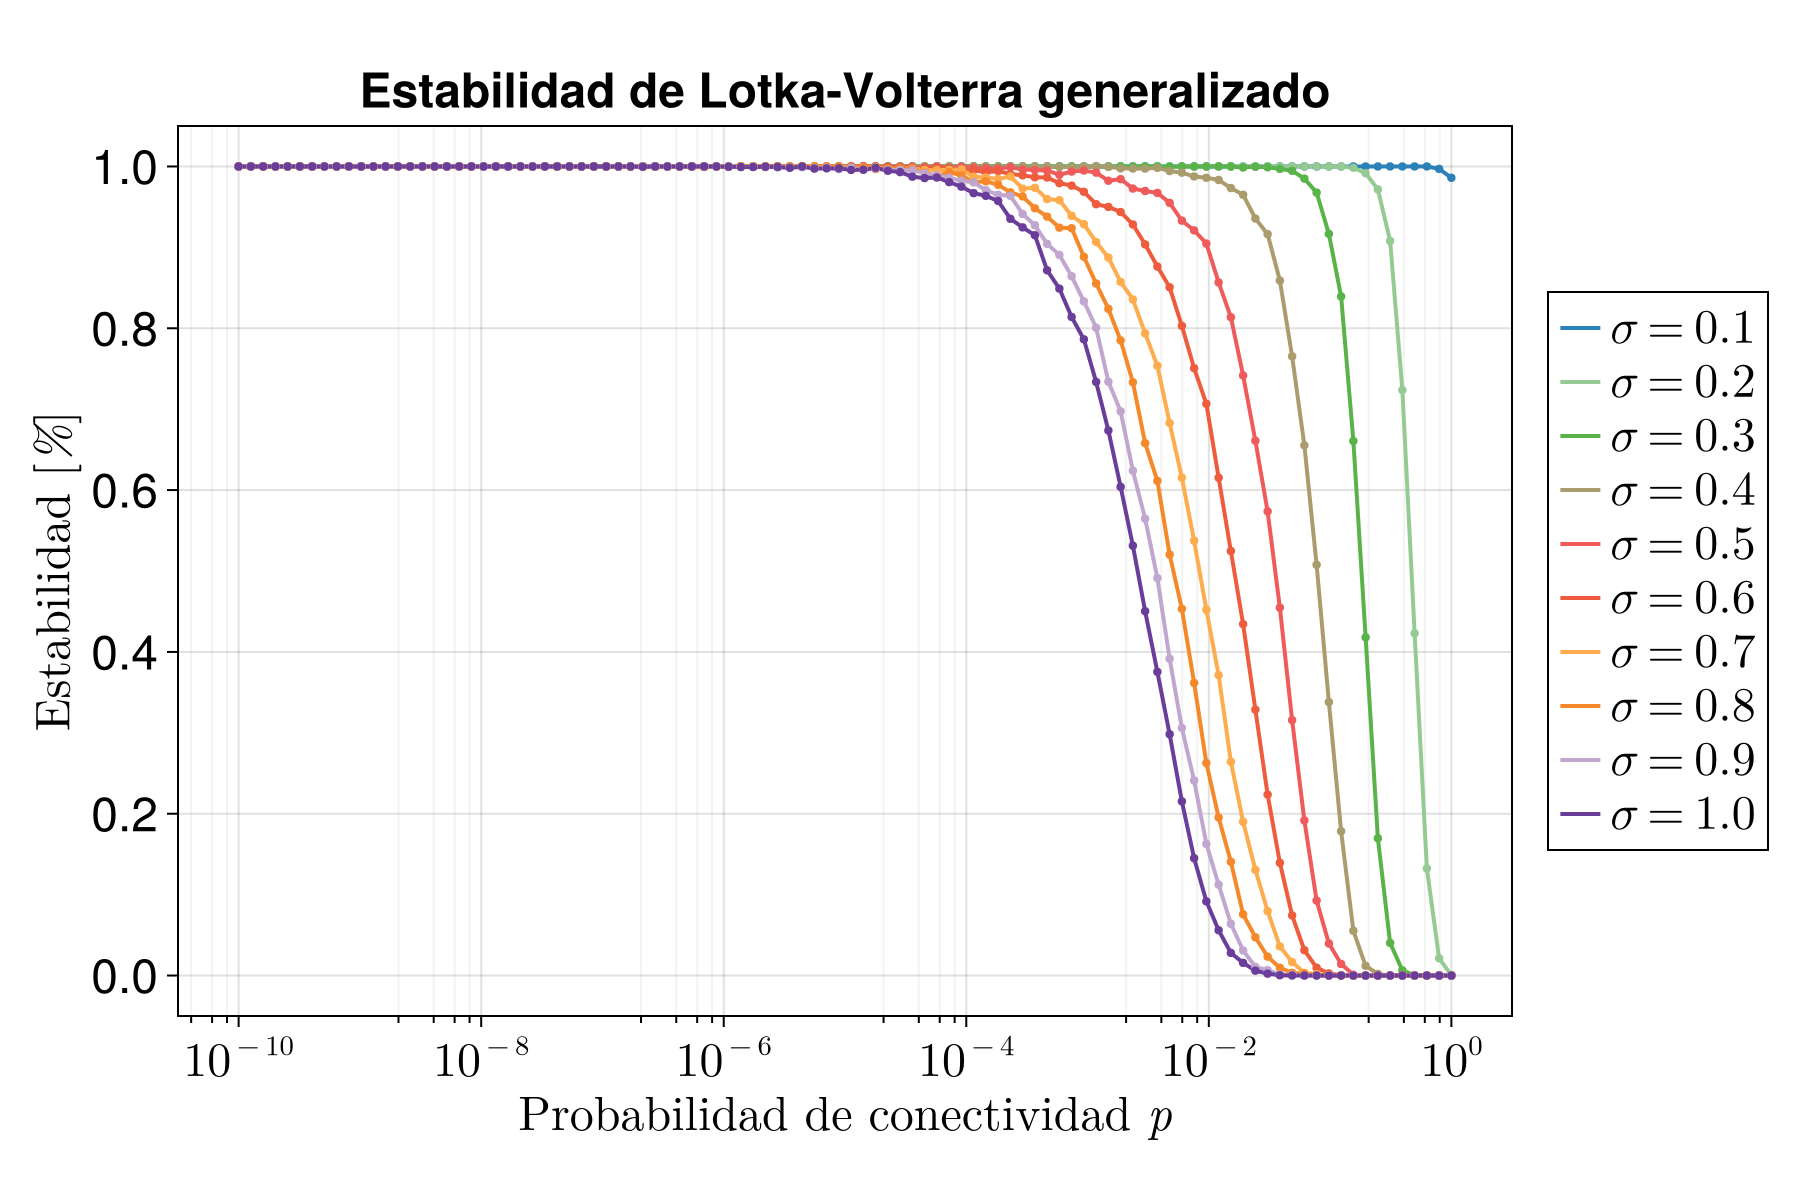
\includegraphics[scale=0.2]{../Imagenes/EstabilidadLKpLog}
	\caption{Transiciones de estabilidad en el Sistema de Lotka-Votlerra generalizado en función de la probabilidad con escala logarítmica para $N=100$.}
	\label{fig:EstabilidadLKpLog}
\end{figure}

A continuación se realizarán una serie de comparaciones entre sistemas de Lotka-Volterra generalizado con $\Lambda$ estructuralmente simétrica y aleatoria, pero también se realizarán comparaciones con respecto de los sistemas de May antes mencionados. En el primer caso para notar cómo es la desviación entre la elección de $\Lambda$ y en el segundo caso para notar la desviación con respecto de sistemas que consideran la diagonal fija.\\
\begin{wrapfigure}{l}{0.5 \textwidth} \vspace{-30pt} \begin{center}
		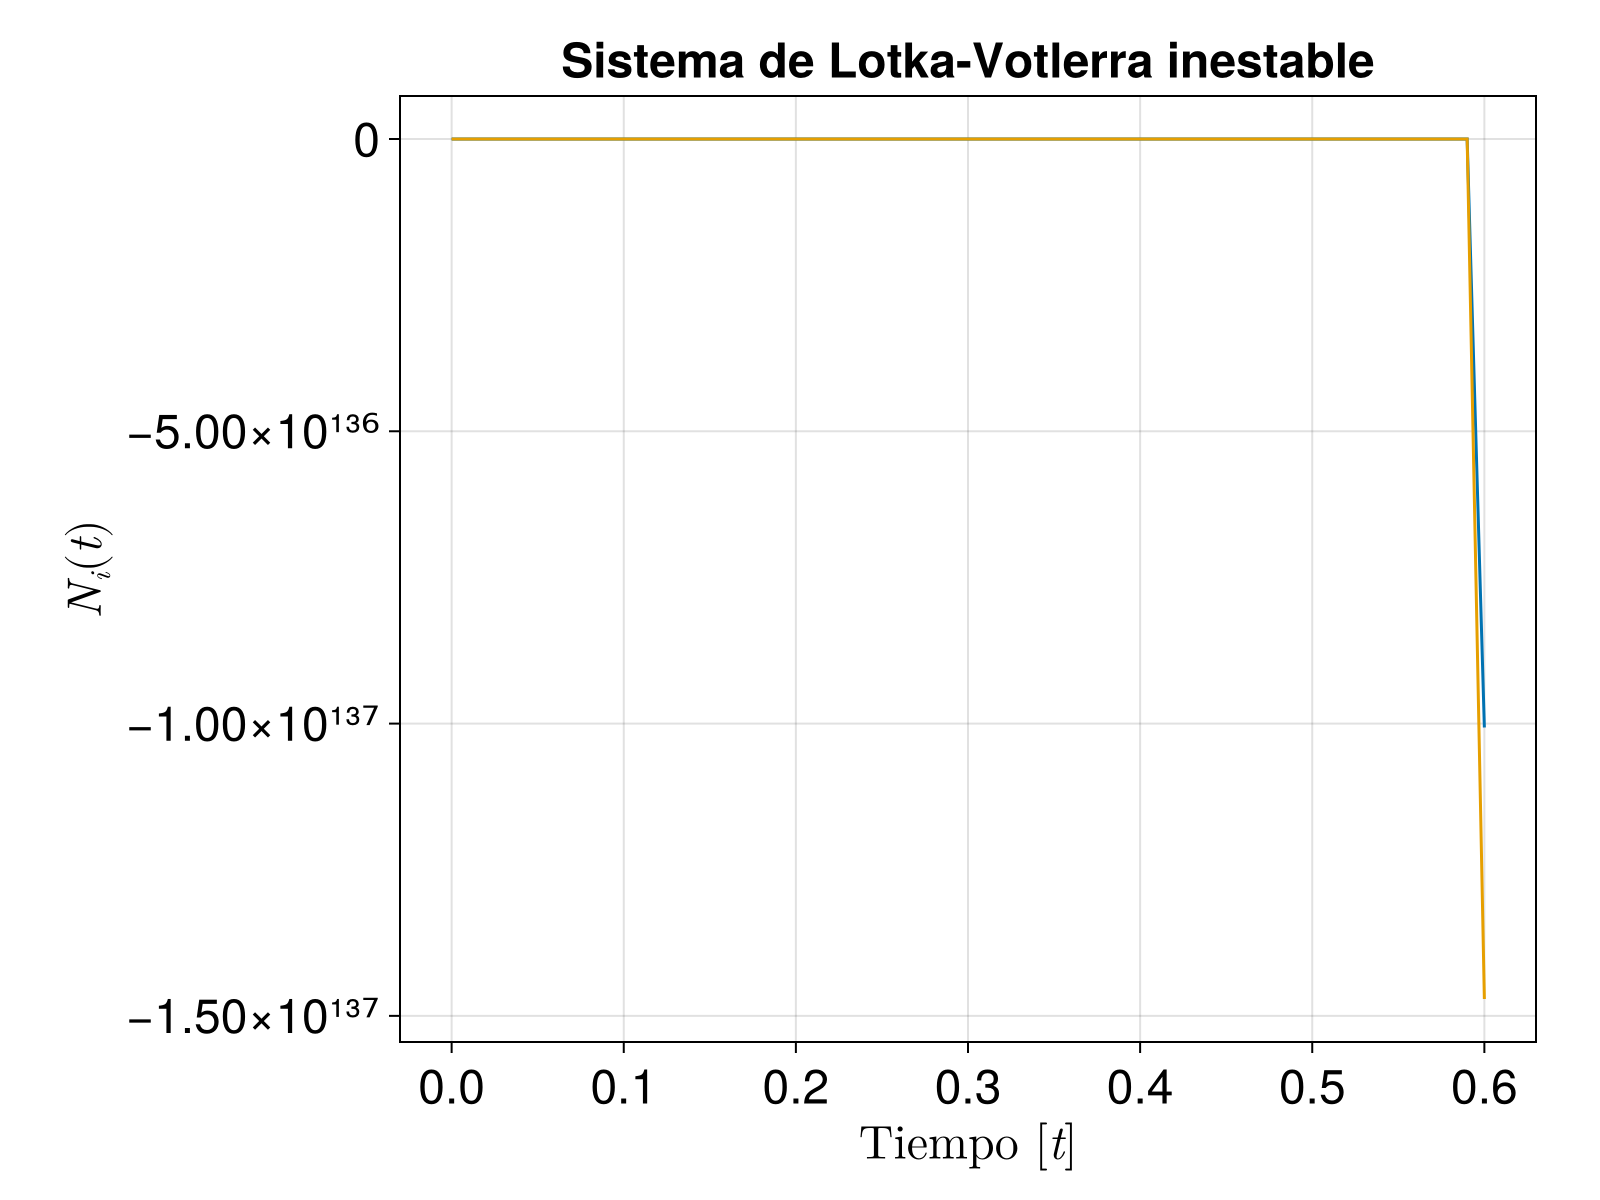
\includegraphics[scale=0.135]{../Imagenes/Heuristico}
	\end{center}
	\vspace{-20pt} 
	\caption{Sistema inestable que no cumple con la relación (\ref{eqn:relacionHeuristica})}
	\vspace{-10pt}
	\label{fig:Heuristico}
\end{wrapfigure}
La suavidad de las transiciones de este caso aún es una pregunta abierta al igual que el parámetro de transición, tendrá que ver necesariamente la simetría estructural de las interacciones. Realizando una exploración heurística sobre esta simetría se ha hallado particularmente para el sistema de $2\times 2$ que las interacciones de cooperación  (ambos coeficientes negativos) deben cumplir la relación:
\begin{equation}\label{eqn:relacionHeuristica}
	\alpha_{ij}>\frac{1}{\alpha_{ji}},\qquad \text{con }i\neq j
\end{equation}
para que el sistema (\ref{eqn:LK}) sea estable. Esto implica que $\alpha_{ij}\alpha_{ji}<1$ y si no se cumplen estas condiciones, el sistema deviene a inestable. En la Figura (\ref{fig:Heuristico}) se ha integrado un sistema que no cumple la desigualdad (\ref{eqn:relacionHeuristica}) para un intervalo de tiempo de 0 a 10, y en apenas unos instantes el sistema se disparó a $-\infty$. Esta puede ser una pista importante para hallar una relación de peso que conlleve a la inestabilidad de sistemas generalizados a $N$ especies. 
\\
\\
Al comparar las transiciones del sistema de Lotka-Volterra generalizado con $\Lambda$ aleatoria y estructuralmente simétrica, se observa que las transiciones decaen primero y de forma suave en el segundo caso con respecto del primero. Esto puede deberse en parte por desigualdad (\ref{eqn:relacionHeuristica}), pues es una condición altamente probable conforme $N$ sea más grande. Sin embargo, hace falta generalizar dicha desigualdad a matrices cuadradas con las características de $\Lambda$ y demostrar que la realción esta inmiscuida en este tipo de escenarios, por lo que por ahora no es enteramente concluyente.
\begin{figure}[h!]
	\centering
	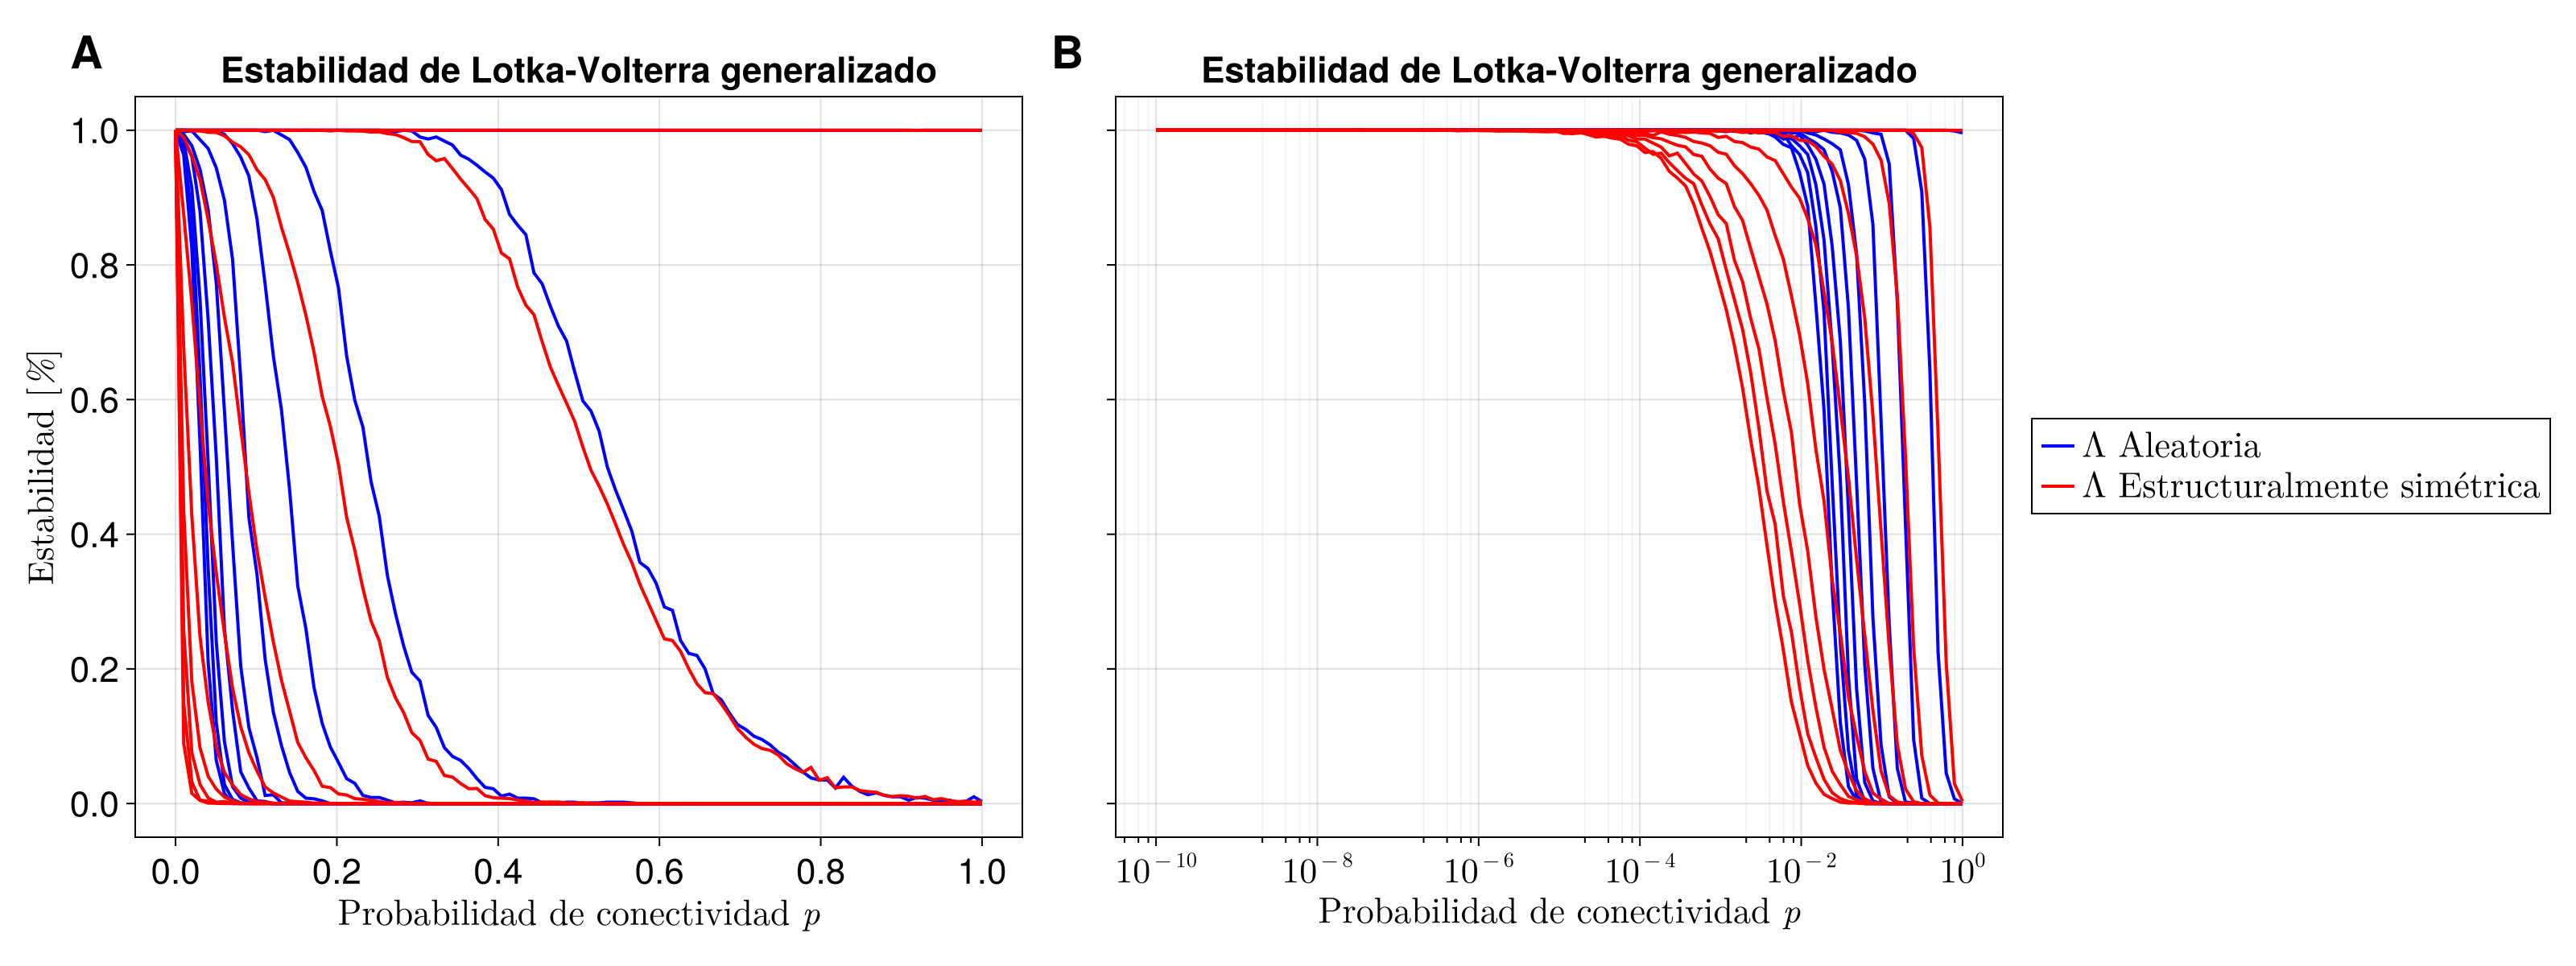
\includegraphics[scale=0.16]{../Imagenes/ComparacionIncidenciasp}
	\caption{Comparación de la estabilidad entre sistemas de Lotka-Volterra generalizados con $\Lambda$ aleatoria y estructuralmente simétrica.}
	\label{fig:ComparacionIncidenciasp}
\end{figure}

Lo que llama la atención es que la desviación es cada vez mayor conforme $\sigma$ aumenta, valores cercanos al cero son más probables que cumplan la desigualdad (\ref{eqn:relacionHeuristica}) que aquellos cercanos a 1. Para notar que distribuciones comienzan a no cumplir la desigualdad, se realiza una simulación que utiliza matrices cuadradas similares a $\Lambda$ solo con la diferencia de que todas sus entradas se mapean de una distribución normal que toma valores discretos tal como en la partición (\ref{eqn:particionSigma}), la simulación considera 3000 matrices por cada $\sigma$ y evalúa cuantos de ellos no cumple la desigualdad. \\
\\
El hallazgo es que a partir de $\sigma=0.27$ se observa la primer distribución normal que no cumple la desigualdad con menos de 10 casos, de ahí en adelante el número de casos no favorables va aumentando hasta $\sigma=1.0$ teniendo hasta una cantidad de 6 cifras de ellos. Y tal cual se nota en la Figura (\ref{fig:ComparacionIncidenciasp}), a partir de $\sigma=0.3$ en adelante se va observando una desviación progresiva hasta $\sigma=1.0$.\\
\\
A partir de esta observación es que se ha relacionado la desigualdad con la estabilidad de los sistemas, tanto de May como el de Lotka-Volterra generalizado. Viendo las diferencias que tiene el sistema (\ref{eqn:LK}) considerando $\Lambda$ estructuralmente simétrica y aleatoria, ahora se mostrará que diferencias existen entre este par de sistemas con los respectivos de May.
\begin{figure}[h!]
\centering
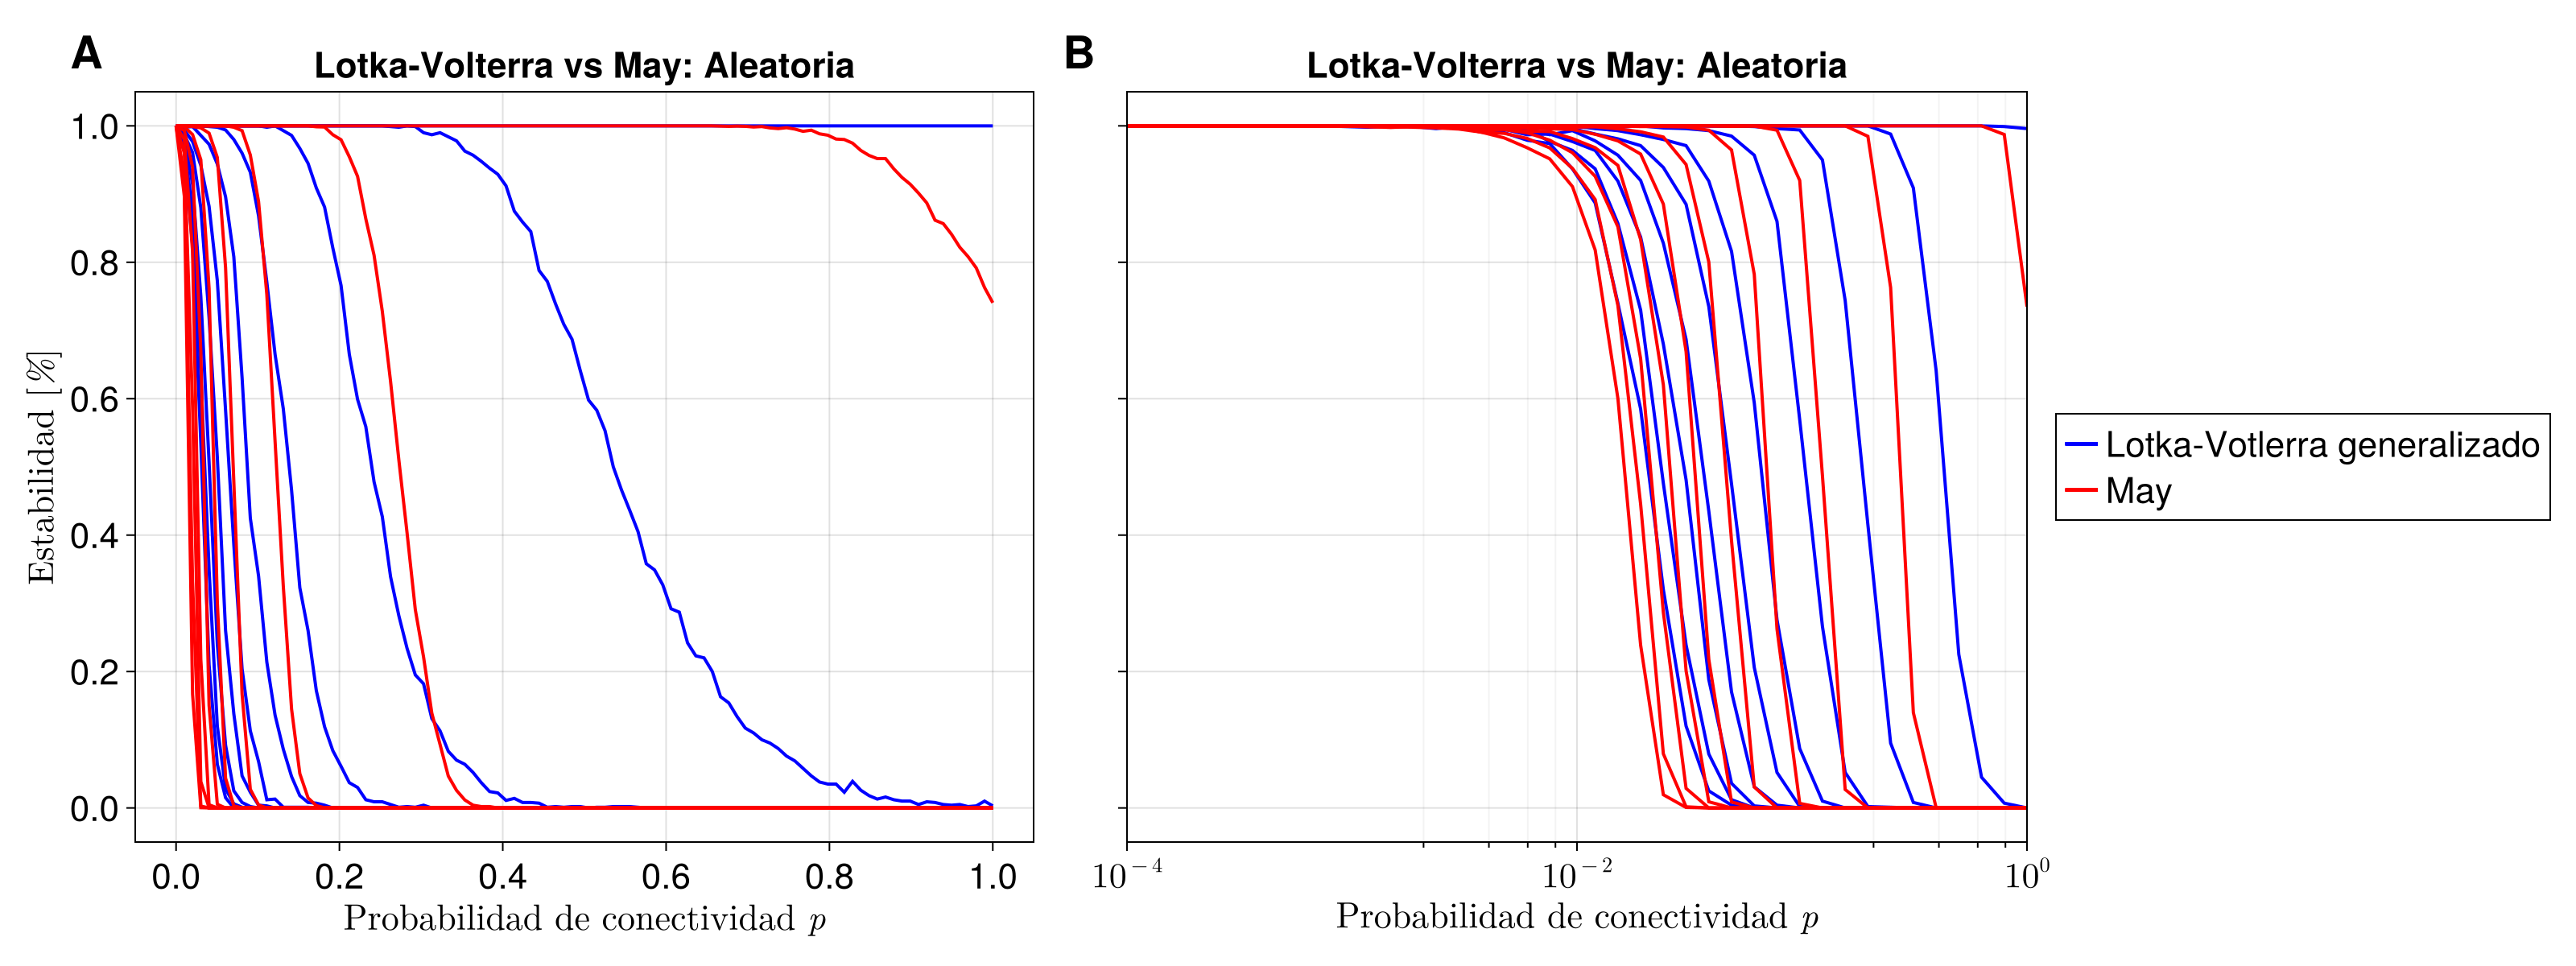
\includegraphics[scale=0.16]{../Imagenes/ComparacionLKMay.png}
\caption{Comparación de la estabilidad entre sistemas de Lotka-Volterra y May en función de $p$ con matrices aleatorias.}
\label{fig:ComparacionLKMay}
\end{figure}

\begin{figure}[h!]
	\centering
	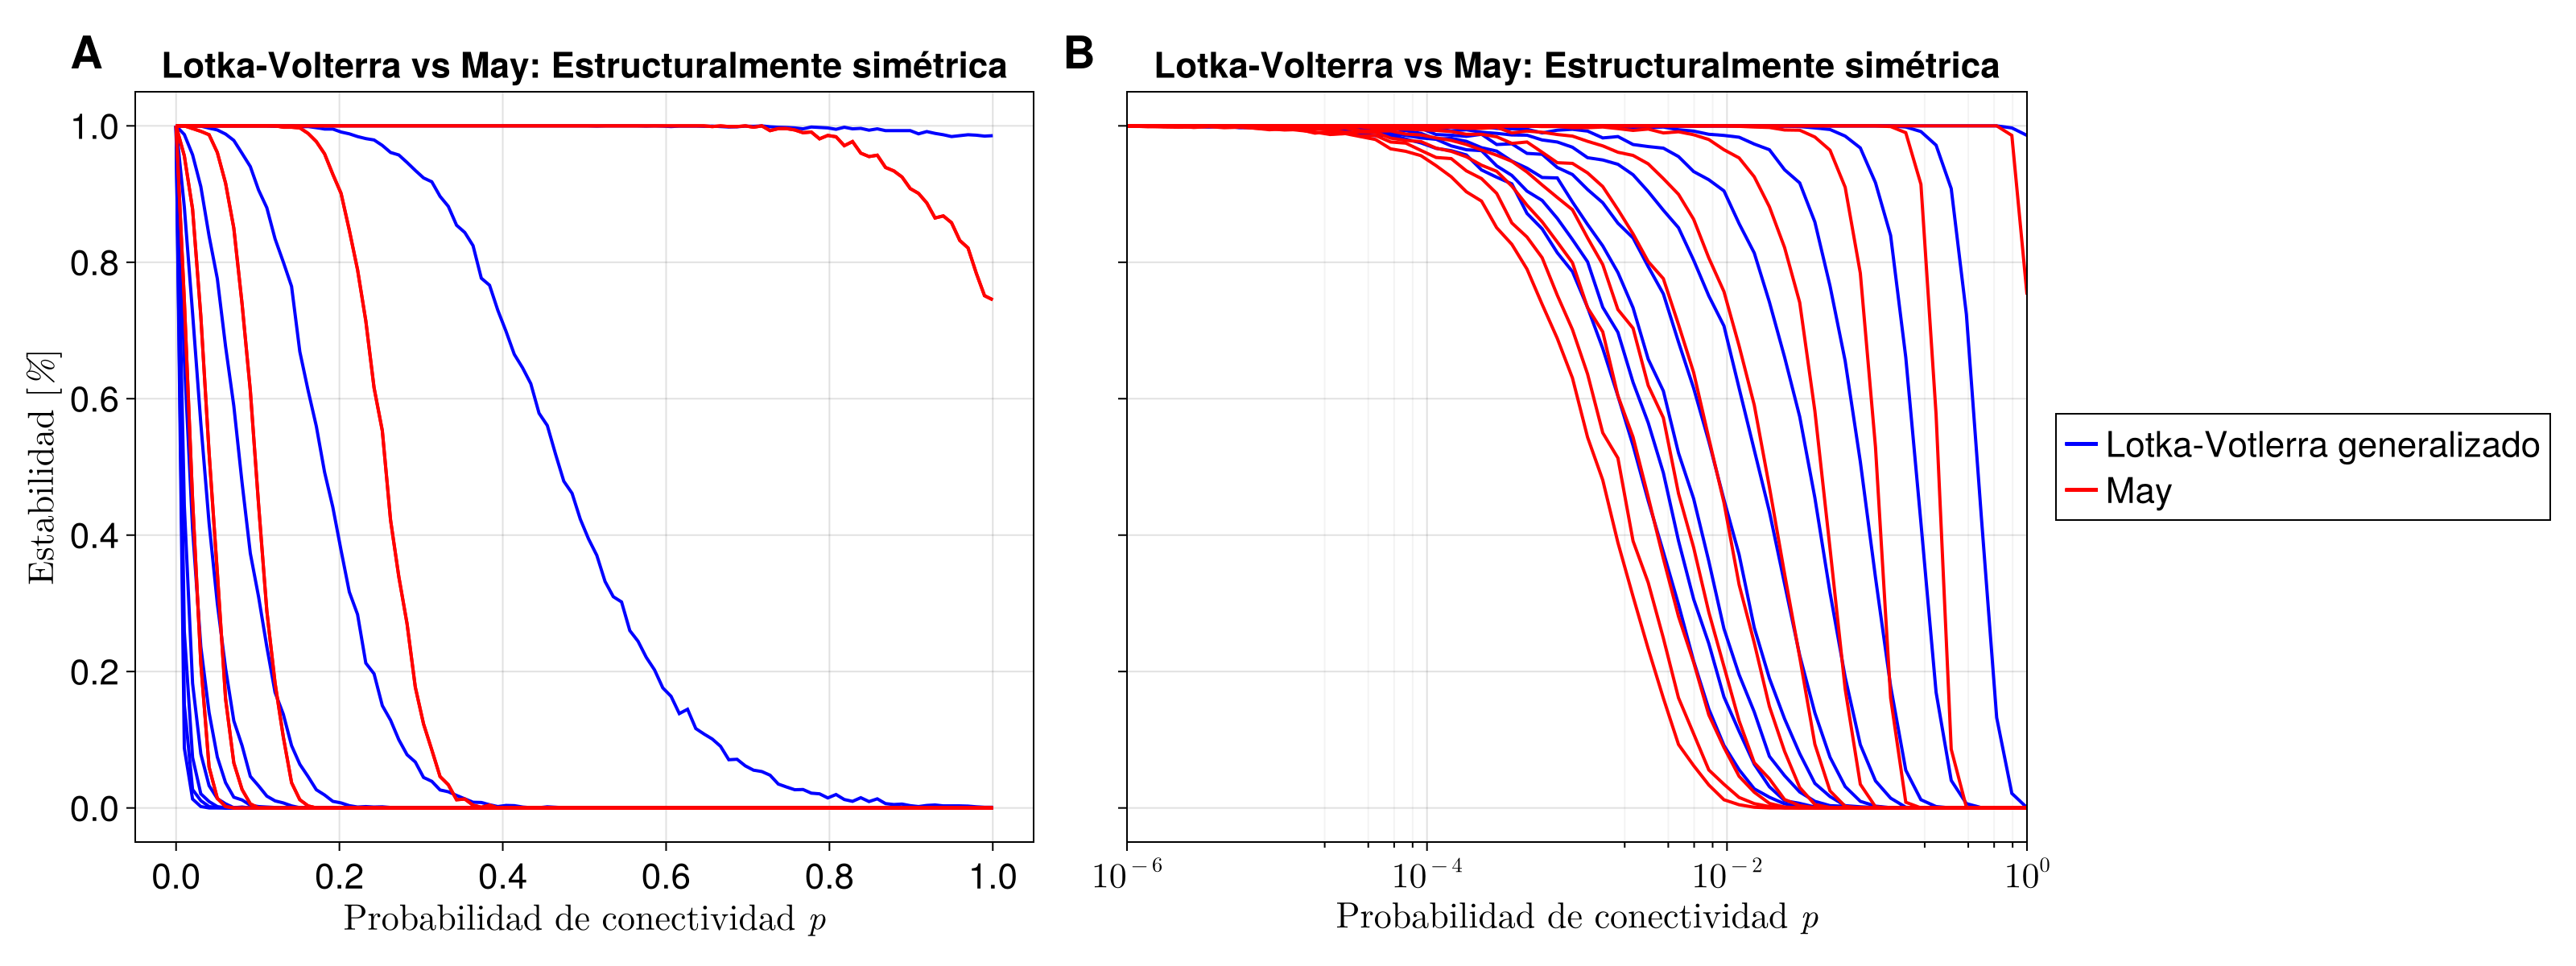
\includegraphics[scale=0.16]{../Imagenes/ComparacionLKMayESim.png}
	\caption{Comparación de la estabilidad entre sistemas de Lotka-Volterra y May en función de $p$ con matrices estructuralmente simétricas.}
	\label{fig:ComparacionLKMayESim}
\end{figure}

En esta ocasión se percibe que la estabilidad de los sistemas de May decaen primero que los de Lotka-Volterra generalizado, para ambos casos distinguiendo entre las matrices aleatorias y estructuralmente simétricas. Además de ello lo hacen de forma similar para $\sigma\geq0.2$; a pesar de ello la diferencia esta presente en la estructura de las matrices jacobianas y las de May, principalmente por el hecho de que están regidas por distribuciones completamente diferentes.

Una suposición válida que se puede derivar de la estructura de las matrices con respecto de la forma de transición de sus estabilidades, es que lo harán en función de la distribución estadística con las que estén formadas. Se podrían formar otro tipo de sistemas con otras distribuciones para poder observar de que forma decaen y si siguen las tendencias que se muestran en las formas aleatorias y estructuralmente simétricas.

\subsubsection*{En función de $\sigma$}

Otra perspectiva que se tiene de la estabilidad del sistema (\ref{eqn:LK}) es utilizando la partición (\ref{eqn:particionSigma}) y ver de que manera cambia considerando varias probabilidad tal y como se mostró anteriormente con los diagramas de transición en función de $p$. Al igual que con las transiciones de May en función de $\sigma$, estas también ocurrirán hacia la derecha con respecto de las transiciones en función de $p$. En el caso de May se le atribuía al hecho de que su parámetro de transición $\sigma^*$ es proporcional a $\frac{1}{\sqrt{N}}$ mientras que $C^*\propto\frac{1}{N}$. Ya se sabe que el parámetro (\ref{eqn:radioMayGirko}) no aplica enteramente a las transiciones de Lotka-Volterra generalizado, sin embargo, podría estar involucrado de alguna forma mediante esta pista.
\begin{figure}[h!]
	\centering
	\includegraphics[scale=0.2]{../Imagenes/EstabilidadLKσLin}
	\caption{Transiciones de estabilidad en el Sistema de Lotka-Volterra generalizado en función de la fuerza de interacción promedio para $N=100$.}
	\label{fig:EstabilidadLKσLin}
\end{figure}

Este escenario en particular puede ayudar a develar la relación entre la estabilidad y la simetría estructural de las interacciones. Al igual que en la Figura (\ref{fig:ComparacionIncidenciasp}), se va a mostrar como cambia la estabilidad cuando se consideran matrices de incidencias $\Lambda$ aleatorias y estructuralmente simétricas. En su caso análogo, se observaba que las transiciones de $\Lambda$ aleatoria se muestra hacia la derecha con respecto de la estructuralmente simétrica. 
\newpage
\begin{figure}[h!]
	\centering
	\includegraphics[scale=0.22]{../Imagenes/ComparacionIncidenciasσ}
	\caption{Comparación de la estabilidad entre sistemas de Lotka-Volterra generalizados en función de $\sigma$ con $\Lambda$ aleatoria y estructuralmente simétrica.}
	\label{fig:ComparacionIncidenciasσ}
\end{figure}

En este caso las transiciones con $\Lambda$ aleatoria también ocurren hacia la derecha de las estructuralmente simétricas, pero a diferencia del caso de la Figura (\ref{fig:ComparacionIncidenciasp}), las desviaciones van disminuyendo conforme la conectividad aumenta, tal y como se observó con el caso de May (Figuras (\ref{fig:TransicionMaySigma} \textbf{B}, \ref{fig:TransicionσDirvsNoDir})). El las transiciones estructuralmente simétricas se logra observar como comienzan a ocurrir desde un rango alrededor del 0.2 al 0.4, lo que empata con la simulación realizada para observar el cumplimiento de la desigualdad (\ref{eqn:relacionHeuristica}). 
\begin{figure}[h!]
	\centering
	\includegraphics[scale=0.16]{../Imagenes/ComparacionLKMayσ}
	\caption{Comparación de la estabilidad entre sistemas de Lotka-Volterra y May en función de $\sigma$ con matrices aleatorias y estructuralmente simétricas.}
	\label{fig:ComparacionLKMayσ}
\end{figure}
\newpage
Para las comparaciones entre sistemas de May y de Lotka-Volterra generalizado, las diferencias son similares a las Figuras (\ref{fig:ComparacionLKMay}, \ref{fig:ComparacionLKMayESim}) en el sentido de que las transiciones de May se notan hacia la izquierda con respecto de las transiciones de Lotka-Volterra. Las formas de transición dependen de la estructura de las matrices que los representan, específicamente hablando de la diagonal: en el caso de May el radio Gershgorin \cite{GershgorinTheorem} y el radio espectral de Girko \cite{girko1985circular} define ``fácilmente'' el punto de transición que para los sistemas de Lokta-Volterra no es tan simple debido a su diagonal heterogénea. 

\subsection{Para $N=50$}

\subsubsection*{En función de $p$}

Se ha utilizado la misma metodología para generar los diagramas de transición para este caso y para $N=25$. Las particiones y los parámetros de (\ref{eqn:LK}) son los mismos. Lo único que ha cambiado es el número de simulaciones por punto (Tabla (\ref{tab:SimulacionesTransicion})), pues entre menos especies se contemplen se debe de compensar con el número de simulaciones para cumplir la ley de los grandes números. Algo que se podrá observar en estas transiciones es que son cada vez más suaves y tienen mayor rango de estabilidad, lo que sugiere que es más probable hallar sistemas estables cuando su tamaño es cada vez menor.
\begin{figure}[h!]
	\centering
	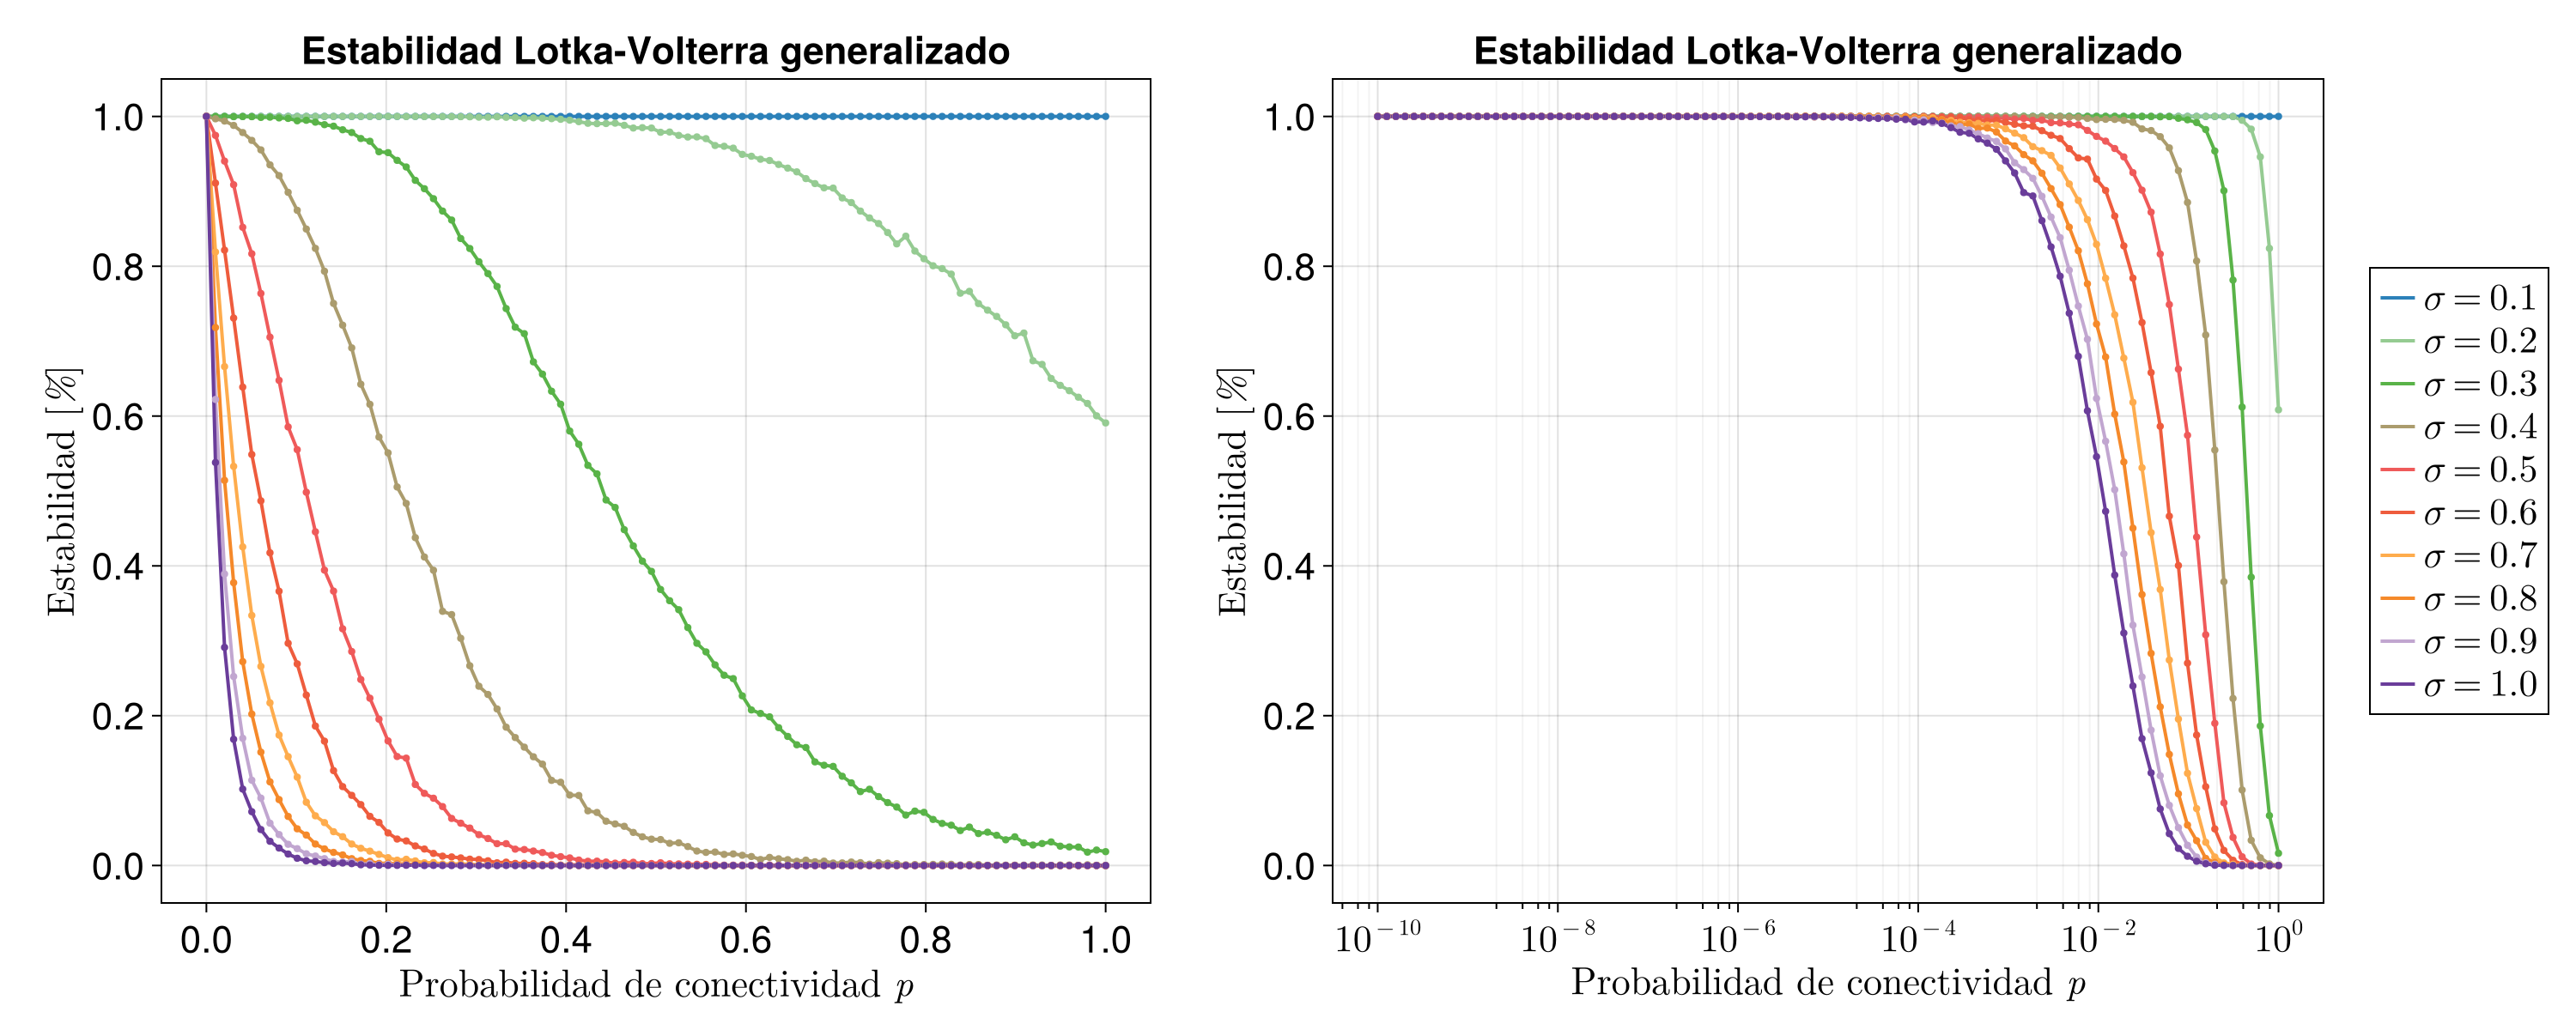
\includegraphics[scale=0.16]{../Imagenes/EstabilidadLKp50}
	\caption{Transiciones de estabilidad en el Sistema de Lotka-Volterra generalizado en función de la probabilidad de conectividad para $N=50$.}
	\label{fig:EstabilidadLKp50}
\end{figure}

Se puede observar sutilmente como el caso $\sigma=0.2$ tiene hasta un 60\% de probabilidad de ser estable aún cuando la red es completamente conectada, hecho que contrasta con el caso $N=100$. Sin embargo aún así se sigue observando  que la estabilidad para $\sigma$ cercana a 1 se da para valores $p$ pequeños, del orden de $10^{-4}$. Si se realiza una simulación como la que se mencionó anteriormente para observar el cumplimiento de la desigualdad (\ref{eqn:relacionHeuristica}) los valores son similares al caso $N=100$, lo que indica que a partir de $\sigma=0.27$ comienzan a emerger casos inestables que no cumplen dicha desigualdad.

\subsubsection*{En función de $\sigma$}

Se podrá observar mejor con el diagrama de transición en función de $\sigma$, únicamente cambiará la forma en que decrece con respecto del sistema $N=100$ siendo para este caso más suave en lugar de abrupto.
\begin{figure}[h!]
	\centering
	\includegraphics[scale=0.2]{../Imagenes/EstabilidadLKσ50}
	\caption{Transiciones de estabilidad en el Sistema de Lotka-Volterra generalizado en función de la fuerza de interacción para $N=50$.}
	\label{fig:EstabilidadLKσ50}
\end{figure}

\subsection{Para $N=25$}

\subsubsection*{En función de $p$}

\begin{figure}[h!]
	\centering
	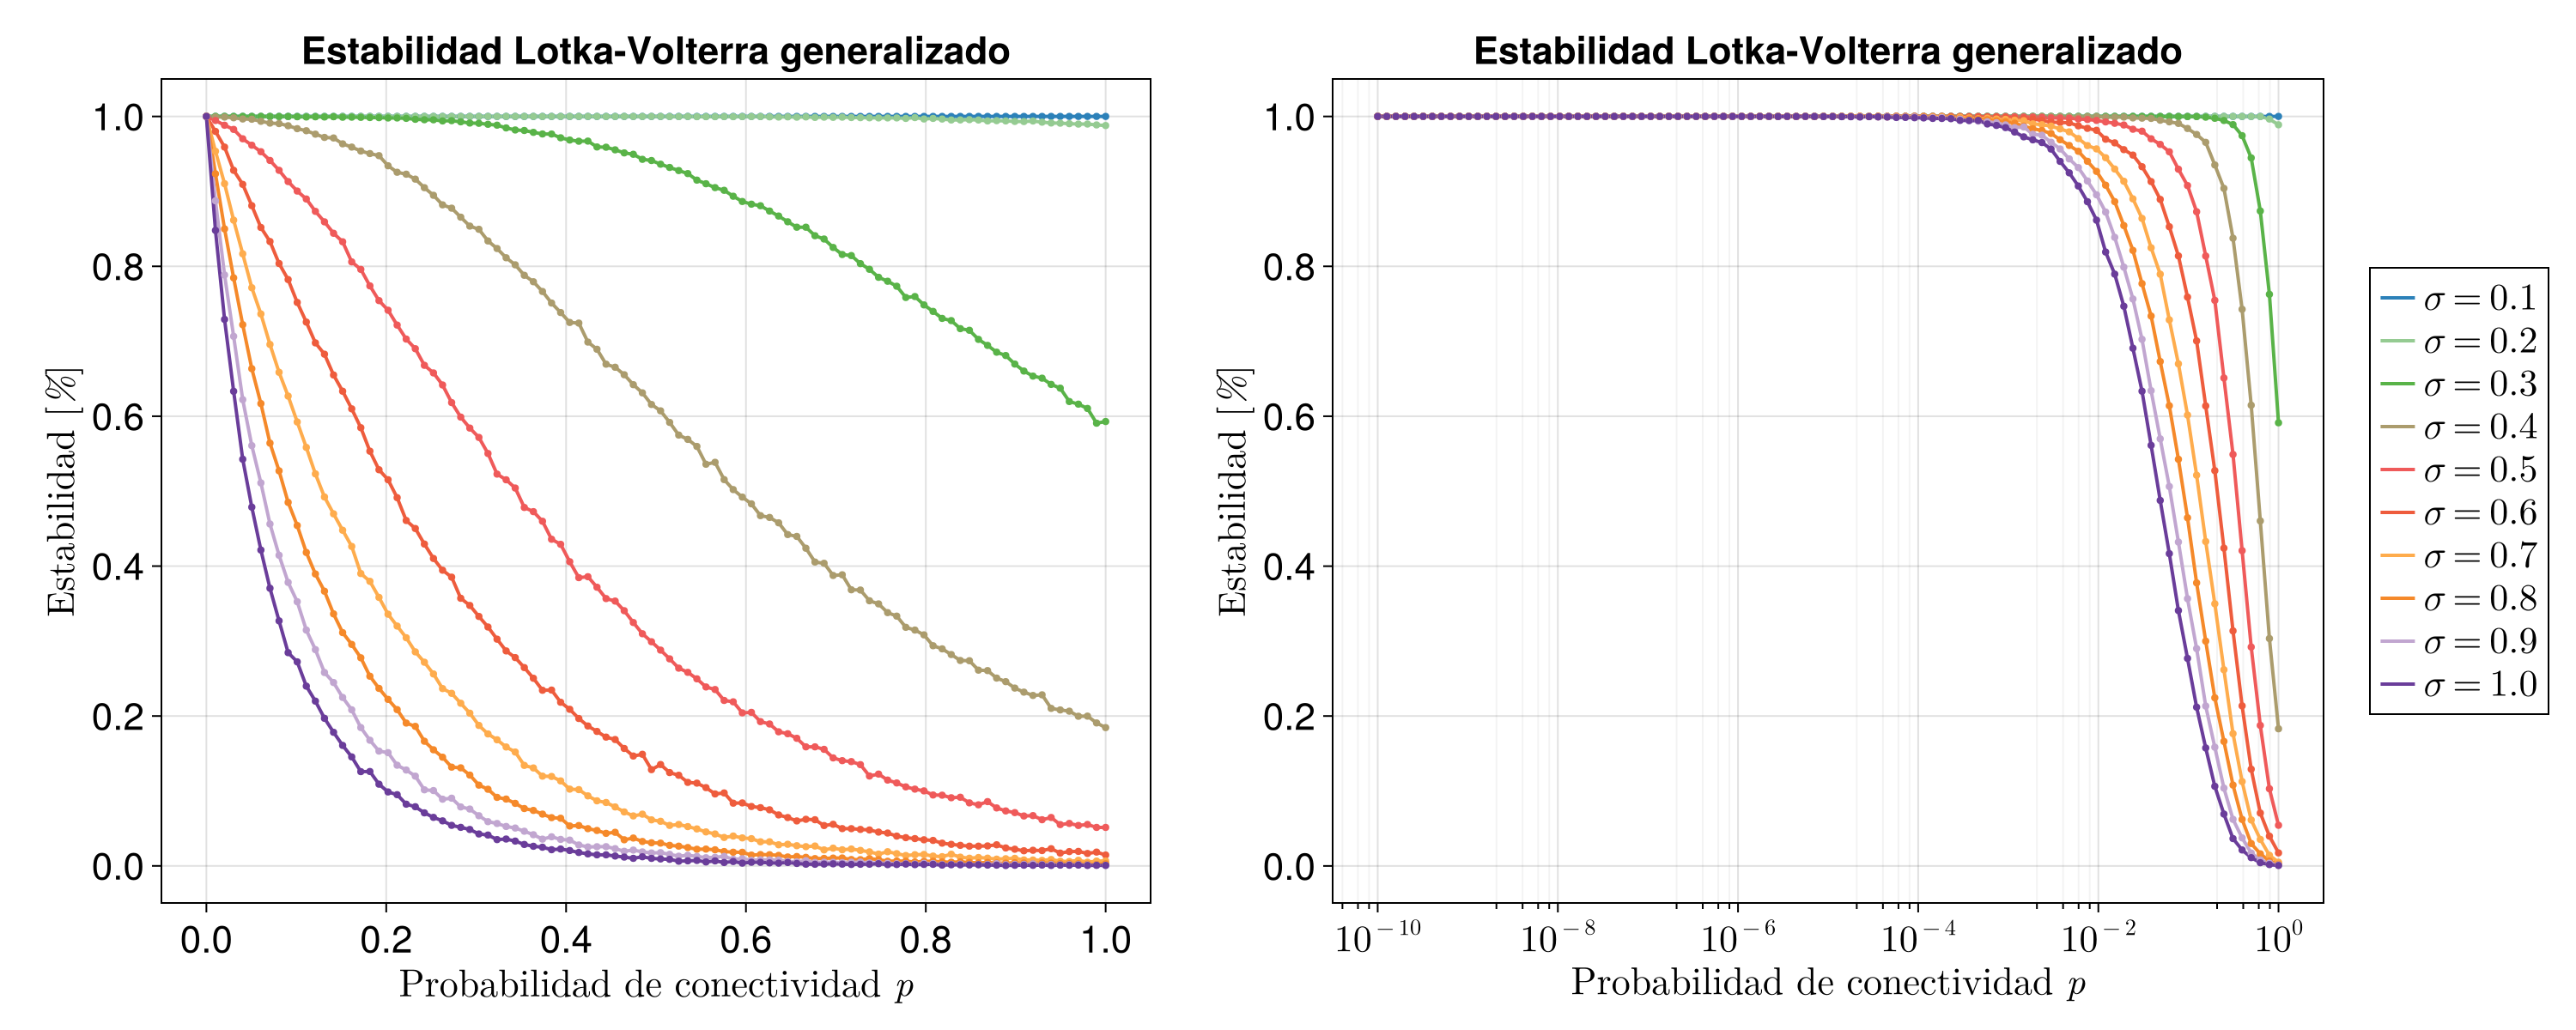
\includegraphics[scale=0.16]{../Imagenes/EstabilidadLKp25}
	\caption{Transiciones de estabilidad en el Sistema de Lotka-Volterra generalizado en función de la probabilidad de conectividad para $N=25$.}
	\label{fig:EstabilidadLKp25}
\end{figure}

Para este último caso se encuentran transiciones de estabilidad todavía más suaves, a su vez con un rango de estabilidad mayor con respecto de los sistemas anteriores. Sin embargo también se contempla un número mayor de simulaciones por punto (Tabla \ref{tab:SimulacionesTransicion}) para poder suavizar las curvas. En este caso se puede observar que el sistema con $\sigma=0.2$ es 99\% estable aún con la red totalmente conexa. En el caso de las transiciones en función de $\sigma$ también se presentan más suaves con respecto de los sistemas anteriores incluso se logra observar para $p=0.1$ que el sistema es estable en un 30\% de probabilidad con $\sigma=1.0$, hecho que no se logró observar en los casos anteriores.
\begin{figure}[h!]
	\centering
	\includegraphics[scale=0.2]{../Imagenes/EstabilidadLKσ25}
	\caption{Transiciones de estabilidad en el Sistema de Lotka-Votlerra generalizado en función de la fuerza de interacción para $N=25$.}
	\label{fig:EstabilidadLKσ25}
\end{figure}

Con esto se concluye la presentación de los resultados más importantes de esta tesis, en este punto se tiene un mapa general de como se comporta la estabilidad en sistemas de Lotka-Volterra generalizado para diversos conjuntos de $p$, $\sigma$ y $N$. Haría falta reconocer si puede existir o no un parámetro crítico de transición además de revisar si la relación (\ref{eqn:relacionHeuristica}) tiene alguna relevancia en dicho parámetro de transición. En la siguiente y última sección de este trabajo se estará discutiendo las posibles implicaciones de esto.
\newpage

\section{Un acercamiento al parámetro crítico}

Existen antecedentes sobre transiciones de fase aplicando el modelo de Lotka-Volterra \cite{bunin2017ecological, biroli2018marginally, altieri2021properties}, específicamente dados en el enfoque de \textit{spin glasees}. Cada uno de los trabajos construye de forma particular el sistema y lo conlleva a resultados interesantes, en esta última sección se explorará brevemente cada enfoque y se abrirá la discusión sobre nuestra transición de fase entre régimen estable de un solo punto de equilibrio al inestable, tal y como se mostró en los diagramas de transición antes presentados.
\\
\\
Para el trabajo aportado por Bunin en 2017 \cite{bunin2017ecological} se consideran las ecuaciones comunes del sistema de Lotka-Volterra (\ref{eqn:LK}) considerando que las interacciones se mapean de forma independiente cumpliendo $\mu\equiv N\langle\alpha_{ij}\rangle$ y $\sigma^2\equiv N\, \Var(\alpha_{ij})$. Además de ello, se define un parámetro $\gamma$ que muestra la correlación entre cada una de las interacciones intervinientes, es decir:
$$\gamma = \text{corr}(\alpha_{ij},\alpha_{ji})\in[-1,1]$$
donde para cada $\gamma\neq 0$ se estará considerando el escenario de Allesina (valores propios distribuidos en una Ley Elíptica), mientras que en $\gamma=0$ se consideran los sistemas dados por May (valores propios distribuidos en una Ley Circular). Bunin propone una reparametrización de las ecuaciones considerando abundancias normalizadas para considerar tamaños relativos de las poblaciones consideradas, por tanto define
$$n_i=\frac{x_i}{\frac{1}{N}\sum_{j=1}^N x_j},\qquad\qquad \frac{1}{S}\sum_i n_i=1$$
Además de definir convenientemente las interacciones de la siguiente manera
$$\alpha_{ij}=\frac{\mu}{S}+\sigma\alpha_{ij}$$
con $\langle a_{ij}\rangle=0$, $\langle a_{ij}^2\rangle=\frac{1}{S}$ y $\langle a_{ij}a_{ji}\rangle=\frac{\gamma}{S}$ y los $a_{ij}$ pueden venir de cualquier distribución estadística que cumpla con dichas media y varianza. Por otro lado se consideran las capacidades de carga $K_i$ provenientes de una distribución normal (tal que $\langle K_i\rangle=1$ y $\sigma_K\equiv\Var(K_i)$) e independientes de las $\alpha_{ij}$, de modo que las $x_i\to x_i/\langle K_i\rangle$. Al explorar las condiciones de equilibrio $\frac{dx_i}{dt}=0$ con base en la reparametrización se obtiene
$$0=n_i\left (\lambda_i - un_i-\sum_{j\neq i}a_{ij}n_j + h\right) $$
considerando las siguientes cantidades: $u=\frac{1-\mu/N}{\sigma}$, $\lambda_i=\frac{K_i-1}{\sigma \langle x_i\rangle}$ y $h=\frac{1}{\langle x_i\rangle}-\frac{\mu}{\sigma}$, además se define $\sigma_\lambda=\Var(\lambda_i)=\frac{\sigma_K^2}{(\sigma\langle x_i\rangle)^2}$. Con esta reparametrización, Bunin establece que el sistema es invariante ante ciertas transformaciones, y toda la información relevante se encuentra contenida en $u$, $\gamma$ y $\sigma_\lambda^2$. Posteriormente se encarga de implementar el \textit{método de cavidad} para hallar la distribución de abundancias y la fracción de especies coexistentes hallando que es una gaussiana truncada
$$n=\max\left (0,\frac{h+\sqrt{q+\sigma_\lambda}z}{u-\gamma v}\right ),\qquad z\sim \mathcal{N}(0,1)$$
donde $\phi$ corresponde con la fracción de especies con $n_i>0$, $q=\langle n_i^2\rangle$ y $v=\langle\partial n_i/\partial \xi_i\rangle$ equivalente a la susceptibilidad. Ello conlleva a determinar la condición crítica de transición entre un único punto de equilibrio a múltiples de ellos, obedeciendo
$$\phi=(u-\gamma v)^2$$
Finalmente concluye que en la fase del único punto de equilibrio, los sistemas ecológicos son predecibles y convergen a dicho punto de equilibrio independientemente de su trayectoria. En la fase de los múltiples puntos fijos, emergen diferentes comunidades con distintas composiciones, dependiendo de condiciones iniciales y el orden de llegada de las especies. La transición se controla gracias a la heterogeneidad de las interacciones y la simetría de la matriz de interacción.\\
\\
Este trabajo continúa y se extiende en 2018 \cite{biroli2018marginally} enfocándose en sistemas de Lotka-Volterra que se encuentran en el borde de la estabilidad, es decir, explorando las implicaciones de un equilibrio marginalmente estable\footnote{Cuando el mínimo valor propio de la matriz Jacobiana es cero}. Las consecuencias de este estado del sistema es que se vuelve extremadamente sensible a perturbaciones, implicando que cualquiera de ellas aleje al sistema de su estabilidad sin que diverga del mismo, sino que más bien lo orbite. Las fluctuaciones pueden ser incluso ambientales (aunque eso recae a interpretación) y amplifican las correlaciones de largo alcance entre especies (en analogía con puntos críticos de transiciones de fase). Esto permite mantener alta diversidad sin perder estructura y refleja un equilibrio entre orden y caos.\\
\\
Más adelante, en 2021 surge una continuación sobre este trabajo pero con un ligero cambio de perspectiva. Altieri \textit{et al.} \cite{altieri2021properties} propone tomar el sistema de Lotka-Volterra generalizado añadiéndole ruido (demográfico) gaussiano\footnote{Correspondiente a nacimientos y decesos que ocurren en las poblaciones.}. El objetivo principal que buscan resolver es ver en que escenarios el tamaño del sistema es susceptible al ruido y como se conecta esto con las fases de tipo \textit{spin glasses}. Para ello definen el sistema de la siguiente manera
\begin{equation}\label{eqn:LKAltieri}
	\frac{dx_i}{dt}=x_i\left( 1-x_i-\sum_{j\neq i}\alpha_{ij}x_j\right )+\eta_i(t)
\end{equation}
Se considera una martiz aleatoria y simétrica con elementos $\alpha_{ij}=\alpha_{ji}$ i.i.d, y $\eta_i(t)$ es el ruido gaussiano con media diferente de cero y con covarianza: $\langle \eta_i(t)\eta'_i(t)\rangle=2TN_i(t)\delta_{ij}\delta(t-t')$ con $T=\frac{1}{N}$; éste término multiplicativo indica que mientras más grande sea la población, menor será el impacto del ruido demográfico sobre el sistema y viceversa; cuando es débil entonces converge a un único punto de equilibrio determinado por los coeficientes de la matriz aleatoria, mientras que cuando el ruido es fuerte las trayectorias generadas no convergen a un punto en especial, sino que se vuelven erráticas y/o atrapadas en zonas metaestables del espacio de estados, lo que conlleva a la fase vítrea.\\
\\
En este contexto la fase vítrea corresponde con una dinámica ecológica lenta, con tiempos de relajación extremadamente largos, atrapada en una jerarquía de valles y subvalles que imposibilita la exploración de todo el espacio posible (ruptura de ergodicidad). Además es altamente dependiente de las condiciones iniciales y del historial de las trayectorias, generando que cualquier perturbación conlleve a otro valle/subvalle; por lo tanto existe una proliferación de estados marginales. Este comportamiento emergerá de la alta heterogeneidad de la matriz aleatoria ($\sigma$) o de la alta intensidad del ruido demográfico reflejado en el tamaño efectivo del sistema.\\
\\
El punto central de las fases consideradas en este trabajo emerge del hecho de poder definir un Hamiltoniano que a su vez define una función de partición. Pensando en ello el sistema sigue una dinámica tipo gradiente descendiente, es decir:
\begin{equation}\label{eqn:Gradiente}
	\frac{dx_i}{dt}=-\frac{\partial H}{\partial x_i}
\end{equation}
Altieri \textit{et al.} establecen que los mínimos locales de la energía del sistema corresponden con los puntos de equilibrio del mismo. Por lo tanto, serán los mínimos de la energía los que describan las fases del sistema de acuerdo con el impacto de $\sigma$ y $T$: si es tal que solo genera un único mínimo, el sistema se organiza en torno al mismo. Al ir aumentando la intensidad de las condiciones mencionadas emergen múltiples puntos de equilibrio y hasta una cantidad exponencial de ellos (fase vítrea) con la cualidad de ser marginalmente estables. \\
\\
Al haber definido un Hamiltoniano asociado al sistema, se puede generar una distribución de estados estacionarios de Boltzmann $P(\{ x_i\})=e^{-\frac{H(\{x_i\})}{T}}$ el cual es posible generar gracias a que el sistema es conservativo\footnote{Cumpliendo
$\frac{\partial}{\partial x_j}\left (\frac{F_i}{x_i}\right )=\frac{\partial}{\partial x_i}\left (\frac{F_j}{x_j}\right )$
con $F_i=-x_i\frac{\partial H}{\partial x_i}$ y al mismo tiempo las $F_i$ son las ecuaciones del sistema (\ref{eqn:LKAltieri}).}. Al dividir por $x_i$ y aplicar la derivada parcial cruzada se llega al siguiente resultado
\begin{equation}\label{eqn:Conservativo}
	\frac{\partial}{\partial x_j}\left (\frac{F_i}{x_i}\right )=-\alpha_{ij},\qquad\frac{\partial}{\partial x_i}\left (\frac{F_j}{x_j}\right )=-\alpha_{ji}
\end{equation}
el cual es verdadero desde que se consideró simétrica a la matriz aleatoria, es decir, $\alpha_{ij}=\alpha_{ji}$ con sus respectivos valores de la distribución estadística considerada. Considerando estos elementos es posible definir una función de partición para explorar el promedio de cantidades observables, pero el espacio de integración se muestra muy complicado además de que se sale de los objetivos del trabajo de investigación. En resumen, los trabajos analizados brevemente hasta ahora tuvieron un enfoque compartido de analizar la dinámica ecológica del sistema (\ref{eqn:LK}) con puntos fijos estables desde una perspectiva estocástica (Altieri \textit{et al.}) y determinista (Bunin \textit{et al.}), y cada uno aportando conclusiones muy valiosas sobre el tema. Lo que seguirá a continuación será la argumentación de esta tesis al considerar el escenario que antecede a los mencionados: la transición del sistema (\ref{eqn:LK}) de puntos fijos estables a inestables.
% Esto entra en contacto con otro concepto que es equivalente pero que ya no voy a incluir por aquí: el análisis de la matriz Hessiana que son las segundas derivadas del Hamiltoniano sobre x_i y x_j, que es en realidad la matriz de interacciones simétrica que consideran en el trabajo. Al ver que sus valores propios son positivos quiere decir que existen mínimos en el Hamiltoniano que llevan a puntos de equilibrio en el sistema; hay que ver cuantos son los mínimos que generan para relacionarlo a la fase que se espera.
\subsection{Discusión}

El gran acierto de Altieri \textit{et al.} en su trabajo antes mencionado, ha sido el hecho de haber restringido las interacciones del sistema (\ref{eqn:LK}) de forma simétrica, es decir, $\alpha_{ij}=\alpha_{ji}$ para toda entrada de su matriz aleatoria\footnote{Que en este trabajo se le ha bautizado como \textit{Matriz de Incidencias}.}. En (\ref{eqn:Conservativo}) se ha observado como las derivadas cruzadas del sistema generan dichos coeficientes que al ser iguales implica que el rotacional del sistema es igual a cero y por lo tanto se puede definir un campo escalar que toma forma de gradiente descendiente (\ref{eqn:Gradiente}). En su trabajo han definido el Hamiltoniano del sistema mismo que induce a una distribución de Boltzmann y a su respectiva función de partición (si es que se requiriera). \\
\\
Lo más importante de estos elementos reunidos (a criterio de este autor) es la forma en que los mínimos del Hamiltoniano representan los puntos fijos (estables) del sistema. En el trabajo se describen distintas fases que no son sino la cantidad de mínimos de energía locales que puede haber en función de la heterogeneidad de las interacciones y el ruido demográfico. En este sentido se puede definir la \textit{Hessiana} del sistema como
\begin{equation}\label{eqn:Hessiana}
	\mathcal{H}_{ij} = \frac{\partial H}{\partial x_i\partial x_j}
\end{equation}
misma que guardará información de la curvatura del Hamiltoniano de tal modo que sus valors propios determinen ``que tan profundos'' son sus mínimos y que tan susceptibles son ante fluctuaciones. Si los valores propios de la matriz Hessiana son positivos, es decir, Re$(\lambda_{\min}(\mathcal{H}))>0$ implica que existe un único mínimo de energía al cual tiende el sistema. Sin embargo, cuando el mínimo valor propio de esta matriz alcanza el cero entonces la curvatura del Hamiltoniano se aplana y emergen modos blandos que representa una estabilidad marginal, de aquí emergen múltiples mínimos de energía y la fase Gardner. Si los valores propios de la Hessiana son negativos, entonces la curvatura del Hamiltoniano pasa a ser cóncava o máxima lo que desenvuelve en un sistema inestable\footnote{Todos aquellos puntos fijos estables o inestables se dan para $\nabla H=0$.}. \\
\\
Esto es crucial ya que en este contexto, la matriz Hessiana es el inverso aditivo de la Jacobiana, es decir, $\mathcal{J}=-\mathcal{H}$\footnote{Solo es posible gracias a que el sistema es conservativo.} indicando que hay una conexión directa entre el soporte espectral de la matriz Jacobiana (que define si las perturbaciones crecen o se mitigan) y la forma de la curvatura del Hamiltoniano (definiendo si el sistema tiene un mínimo o varios mínimos marginales). En ese sentido el mínimo valor propio de la Hessiana equivale al máximo valor propio de la Jacobiana. En el segundo caso, se considera que mientras Re$(\lambda_{\max}(\mathcal{J}))<0$, el sistema será estable; en cambio cuando es igual a cero se ingresa al terreno de la estabilidad marginal y cuando es positivo el sistema se vuelve inestable.
\newpage
Al intentar determinar las derivadas cruzadas del sistema (\ref{eqn:LK}) considerando que la matriz de incidencias $\Lambda$ es únicamente estructuralmente simétrica se encuentra
$$\frac{\partial}{\partial x_j}\left (\frac{F_i}{x_i}\right )=-\frac{r_i\alpha_{ij}}{K_i},\qquad\frac{\partial}{\partial x_i}\left (\frac{F_j}{x_j}\right )=-\frac{r_j\alpha_{ji}}{K_j}$$
considerando que todas las capacidades de carga $K_i$ y todas las tasas de crecimiento $r_i$ son iguales (en esta tesis) aún así $\alpha_{ij}\neq\alpha_{ji}$ y por lo tanto no se puede definir un campo escalar que represente a la energía del sistema: esta configuración es \textit{no conservativa} y en este caso no puede definirse la Hessiana del sistema. Sin embargo, aún la matriz Jacobiana posee el borde espectral que define la estabilidad del sistema, donde Re$(\lambda_{\max}(\mathcal{J}))=0$ es su frontera.
\\
\\
Ya que el sistema de este trabajo es no conservativo, el tipo de transición que se estará por argumentar no sigue la clasificación de Ehrenfest puesto que no se encuentra definida la segunda derivada de la energía libre, únicamente queda el análisis espectral de la matriz Jacobiana del sistema. Esto implica que se estará hablando de una \textit{transición de fase fuera de equilibrio} ya que las cantidades macroscópicas del sistema (principalmente la energía) no se mantienen constantes en el tiempo, sino que existe un flujo o intercambio de energía dentro del mismo. \\
\\
Para esta y toda transición de fase, es necesario definir sus elementos: El parámetro de control será la probabilidad de conectividad $p$ y/o la fuerza de las interacciones dada por $\sigma$. Se puede armar un parámetro de control conjunto como el de May (\ref{eqn:paramMay}) pero para ello se deberá definir el radio espectral de la distribución de valores propios el cual se discutirá más adelante. El parámetro crítico de transición será aquel punto mencionado Re$(\lambda_{\max}(\mathcal{J})=0)$ y las condiciones del parámetro de control para obtener una estabilidad marginal. Por último el parámetro de orden: será el porcentaje de estabilidad del sistema que cambiará cualitativamente a medida que transite hacia el parámetro crítico, manteniendo una fase ordenada (estable) y otra desordenada (inestable).\\
\\
Como se ha mencionado anteriormente, la diferencia entre un sistema conservativo y uno no conservativo es que en el primero las cantidades macroscópicas, especialmente la energía, se estabilizan y dejan de cambiar en el tiempo, a diferencia del no conservativo que puede llegar a estabilizarse a costa de constantes flujos o intercambios de energía que bien podrían venir desde el exterior del sistema. En esta tesis no se ha mencionado nada acerca de los integrantes del sistema, es decir, no se ha especificado de que especies son y su contribución dentro de la cadena trófica, por ello no se hablarán de flujos externos de energía hacia el sistema, pero si se podrá hablar del flujo de energía a causa de la simetría de las interacciones.
\newpage
El trasfondo conceptual de que las interacciones sean simétricas, es decir $\alpha_{ij}=\alpha_{ji}$, es el efecto que ejerce la especie $x_i$ sobre $x_j$ es la misma en sentido opuesto, eso implica la generación de una función de energía como se ha visto antes. Eso significa que no hay ciclos de flujos netos\footnote{La energía fluye en una dirección preferencial sin que exista una compensación exacta en sentido inverso.} que generen disipación de energía y se genera una tendencia hacia el equilibrio termodinámico. En contraste con el caso estructuralmente simétrico, las interacciones no necesariamente son iguales ($\alpha_{ij}\neq\alpha_{ji}$), entonces de aquí si pueden generarse ciclos de flujos netos: En la depredación una de las especies pierde biomasa mientras que otra la gana, en la competencia desigual una de las especies puede tener ventaja sobre la otra, en el mutualismo una de las especies puede beneficiarse más sobre la otra; por lo tanto gracias a este flujo de energía en dirección preferencial el sistema de Lotka-Volterra no conservativo se concibe \textit{fuera del equilibrio termodinámico}.\\
\\
Durante la tesis se ha mencionado que el soporte espectral define estabilidad del sistema; pero además de ello ¡también definirá su transición de fase! Anteriormente se ha revisado que el sistema de May obedece una Ley Circular que esta sustentada por el trabajo espectral de Girko: el centro del disco esta fijado en el valor constante $-d$ que tiene la diagonal de sus matrices aleatorias y el tamaño del radio espectral obedece (\ref{eqn:radioMayGirko}). Sin embargo, las matrices Jacobianas resultantes de resolver el sistema (\ref{eqn:LK}) tienen una diagonal heterogénea dadas por una distribución de cola pesada con sesgo negativo. Aunque se quisiera determinar un ajuste de la Ley Circular de Girko contemplando las $N$ Leyes Circulares propuestas en la Fig. (\ref{fig:LeyesCirculares}), no sería adecuado ya que los parámetros $\sigma$ y $p$ no inciden directamente sobre la Jacobiana sino sobre la matriz de Incidencias $\Lambda$.\\
\\
Anteriormente se ha observado que la distribución espectral de valores propios no sigue una forma simétrica, sino que es amorfa ajustándose a $N$ círculos. Por esta razón es probable que el radio espectral que defina la transición de fase no sea fácil de determinar. En la sección (\ref{subsec:PuntosFijos}) se han introducido las ideas para poder llegar al objetivo. Lo que se plantea es que las interacciones de la matriz de incidencias $\Lambda$: definen la estabilidad del punto fijo. Por lo tanto la misión es hallar las condiciones $(p,\sigma,N)$ tal que la solución del sistema (\ref{eqn:PuntoFijo}) induzca un punto fijo estable. Esta tarea no es trivial de resolver, pues el sistema tiene al menos $N$ soluciones diferentes y no se sabe de su estabilidad hasta que se evalúe en la Jacobiana. La relación heurística comentada anteriormente (\ref{eqn:relacionHeuristica}) puede ser una pista dentro de esta búsqueda pero por ahora se dejará como un problema abierto que llega al límite de esta tesis.
\newpage
\subsubsection*{Interpretación ecológica}

Al considerar matrices estructuralmente simétricas se esta restringiendo al sistema con la condición de que toda especie tena una de tres interacciones posibles ($++$, $--$, $+-$, $-+$). Esto implica que exista una dirección preferencial en el flujo de energía, pues las interacciones no son balanceadas. En este sentido, el sistema se estabilizará cuando el acoplamiento de todas las interacciones resulte en una configuración ordenada y el meollo del asunto es poder caracterizar dicha configuración con base en parámetro de control (acoplamiento de $(p,\sigma, N)$) aplicado a $\Lambda$. En este aspecto, sería interesante poder explorar si el flujo de energía neta (dadas por las interacciones) esta relacionado con la estabilidad del sistema.\\
\\
Hasta ahora se puede interpretar de manera directa las diferentes fases de estabilidad (al menos matemáticamente) pero físicamente ¿qué es lo que representan? Para el caso de la estabilidad es un punto $N$-dimensional al que todas las especies del sistema llegan y perduran, estos puntos son resistentes ante perturbaciones, cualquiera de ellas las puede mitigar con el tiempo hasta volver a alcanzar su punto estable. En el caso del régimen marginalmente estable representa el punto crítico en que las especies comienzan a ser sensibles en presencia de fluctuaciones y no vuelven a su punto estable pero tampoco divergen, más bien presentan un comportamiento oscilatorio cerca del punto fijo. \\
\\
En el caso de la inestabilidad, matemáticamente representa la sensibilidad que tiene el sistema a ser pertubado y diverger. Pero físicamente las poblaciones no crecen exponencialmente; este caso representa que la especie ya no tiene la capacidad de volver a su punto estable. Dependerá de que tan conectada se encuentre esta especie ``inestable'' para trasmitir ese comportamiento al resto del sistema, y eso dependerá de su grado. El modelo de red aleatoria descrita por una distribución de grado binomial implica de alguna manera las especies están relacionadas íntimamente de forma directa o indirecta, por lo que si al menos una especie no logra regresar a su punto estable entonces eso desencadena en la inestabilidad del sistema completo.\\
\\
Una de las observaciones de los diagramas de transición antes presentados, es que es más probable tener configuraciones ordenadas cuando el número de especies $N$ es cada vez menor...
\newpage
\section{Conclusiones}

En esta tesis se ha investigado sobre la estabilidad del sistema de Lotka-Volterra generalizado abarcando desde su construcción hasta su integración y sus implicaciones con el fin de entender los mecanismos que determinan la persistencia o colapso del sistema. Se ha encontrado que la distribución del punto fijo tiene cola pesada con sesgo positivo. Esto indica que existen pocas especies dominantes que prosperan más que el resto de especies del sistema. La distribución del punto fijo induce a la diagonal de las matrices Jacobianas con la diferencia que ahora tiene sesgo negativo. En este sentido, el soporte espectral de las Jacobianas estará controlado por cada una de los valores de su diagonal generando un conjunto de $N$ Leyes Circulares. Finalmente la estabilidad estará dominada por la tupla $(p,\sigma,N)$ que induce puntos fijos estables en la matriz de incidencias $\Lambda$. \\
\\
